% Template for PLoS
% Version 3.5 March 2018
%
% % % % % % % % % % % % % % % % % % % % % %
%
% -- IMPORTANT NOTE
%
% This template contains comments intended 
% to minimize problems and delays during our production 
% process. Please follow the template instructions
% whenever possible.
%
% % % % % % % % % % % % % % % % % % % % % % % 
%
% Once your paper is accepted for publication, 
% PLEASE REMOVE ALL TRACKED CHANGES in this file 
% and leave only the final text of your manuscript. 
% PLOS recommends the use of latexdiff to track changes during review, as this will help to maintain a clean tex file.
% Visit https://www.ctan.org/pkg/latexdiff?lang=en for info or contact us at latex@plos.org.
%
%
% There are no restrictions on package use within the LaTeX files except that 
% no packages listed in the template may be deleted.
%
% Please do not include colors or graphics in the text.
%
% The manuscript LaTeX source should be contained within a single file (do not use \input, \externaldocument, or similar commands).
%
% % % % % % % % % % % % % % % % % % % % % % %
%
% -- FIGURES AND TABLES
%
% Please include tables/figure captions directly after the paragraph where they are first cited in the text.
%
% DO NOT INCLUDE GRAPHICS IN YOUR MANUSCRIPT
% - Figures should be uploaded separately from your manuscript file. 
% - Figures generated using LaTeX should be extracted and removed from the PDF before submission. 
% - Figures containing multiple panels/subfigures must be combined into one image file before submission.
% For figure citations, please use "Fig" instead of "Figure".
% See http://journals.plos.org/plosone/s/figures for PLOS figure guidelines.
%
% Tables should be cell-based and may not contain:
% - spacing/line breaks within cells to alter layout or alignment
% - do not nest tabular environments (no tabular environments within tabular environments)
% - no graphics or colored text (cell background color/shading OK)
% See http://journals.plos.org/plosone/s/tables for table guidelines.
%
% For tables that exceed the width of the text column, use the adjustwidth environment as illustrated in the example table in text below.
%
% % % % % % % % % % % % % % % % % % % % % % % %
%
% -- EQUATIONS, MATH SYMBOLS, SUBSCRIPTS, AND SUPERSCRIPTS
%
% IMPORTANT
% Below are a few tips to help format your equations and other special characters according to our specifications. For more tips to help reduce the possibility of formatting errors during conversion, please see our LaTeX guidelines at http://journals.plos.org/plosone/s/latex
%
% For inline equations, please be sure to include all portions of an equation in the math environment.  For example, x$^2$ is incorrect; this should be formatted as $x^2$ (or $\mathrm{x}^2$ if the romanized font is desired).
%
% Do not include text that is not math in the math environment. For example, CO2 should be written as CO\textsubscript{2} instead of CO$_2$.
%
% Please add line breaks to long display equations when possible in order to fit size of the column. 
%
% For inline equations, please do not include punctuation (commas, etc) within the math environment unless this is part of the equation.
%
% When adding superscript or subscripts outside of brackets/braces, please group using {}.  For example, change "[U(D,E,\gamma)]^2" to "{[U(D,E,\gamma)]}^2". 
%
% Do not use \cal for caligraphic font.  Instead, use \mathcal{}
%
% % % % % % % % % % % % % % % % % % % % % % % % 
%
% Please contact latex@plos.org with any questions.
%
% % % % % % % % % % % % % % % % % % % % % % % %

\documentclass[10pt,letterpaper]{article}
\usepackage[top=0.85in,left=2.75in,footskip=0.75in]{geometry}

% amsmath and amssymb packages, useful for mathematical formulas and symbols
\usepackage{amsmath,amssymb}

% Use adjustwidth environment to exceed column width (see example table in text)
\usepackage{changepage}

% Use Unicode characters when possible
\usepackage[utf8x]{inputenc}

% textcomp package and marvosym package for additional characters
\usepackage{textcomp,marvosym}

% cite package, to clean up citations in the main text. Do not remove.
\usepackage{cite}

% Use nameref to cite supporting information files (see Supporting Information section for more info)
\usepackage{nameref,hyperref}

% line numbers
\usepackage[right]{lineno}

% ligatures disabled
\usepackage{microtype}
\DisableLigatures[f]{encoding = *, family = * }

% color can be used to apply background shading to table cells only
\usepackage[table]{xcolor}

% array package and thick rules for tables
\usepackage{array}

% multirow for multiple row tables. 
\usepackage{multirow}

% create "+" rule type for thick vertical lines
\newcolumntype{+}{!{\vrule width 2pt}}

% create \thickcline for thick horizontal lines of variable length
\newlength\savedwidth
\newcommand\thickcline[1]{%
  \noalign{\global\savedwidth\arrayrulewidth\global\arrayrulewidth 2pt}%
  \cline{#1}%
  \noalign{\vskip\arrayrulewidth}%
  \noalign{\global\arrayrulewidth\savedwidth}%
}

% \thickhline command for thick horizontal lines that span the table
\newcommand\thickhline{\noalign{\global\savedwidth\arrayrulewidth\global\arrayrulewidth 2pt}%
\hline
\noalign{\global\arrayrulewidth\savedwidth}}


% Remove comment for double spacing
%\usepackage{setspace} 
%\doublespacing

% Text layout
\raggedright
\setlength{\parindent}{0.5cm}
\textwidth 5.25in 
\textheight 8.75in

% Bold the 'Figure #' in the caption and separate it from the title/caption with a period
% Captions will be left justified
\usepackage[aboveskip=1pt,labelfont=bf,labelsep=period,justification=raggedright,singlelinecheck=off]{caption}
\renewcommand{\figurename}{Fig}

% Use the PLoS provided BiBTeX style
\bibliographystyle{plos2015}

% Remove brackets from numbering in List of References
\makeatletter
\renewcommand{\@biblabel}[1]{\quad#1.}
\makeatother



% Header and Footer with logo
\usepackage{lastpage,fancyhdr,graphicx}
\usepackage{epstopdf}
%\pagestyle{myheadings}
\pagestyle{fancy}
\fancyhf{}
%\setlength{\headheight}{27.023pt}
%\lhead{\includegraphics[width=2.0in]{PLOS-submission.eps}}
\rfoot{\thepage/\pageref{LastPage}}
\renewcommand{\headrulewidth}{0pt}
\renewcommand{\footrule}{\hrule height 2pt \vspace{2mm}}
\fancyheadoffset[L]{2.25in}
\fancyfootoffset[L]{2.25in}
\lfoot{\today}

%% Include all macros below

\newcommand{\lorem}{{\bf LOREM}}
\newcommand{\ipsum}{{\bf IPSUM}}

%% END MACROS SECTION


\begin{document}
\vspace*{0.2in}

% Title must be 250 characters or less.
\begin{flushleft}
{\Large
\textbf\newline{Joint modelling of aggregated incidence data and point prevalence surveys for malaria mapping} % Please use "sentence case" for title and headings (capitalize only the first word in a title (or heading), the first word in a subtitle (or subheading), and any proper nouns).
}
\newline
% Insert author names, affiliations and corresponding author email (do not include titles, positions, or degrees).
\\
Tim C.D. Lucas*\textsuperscript{1}, Anita Nandi\textsuperscript{1}, Michele Nguyen\textsuperscript{1}, Susan Rumisha \textsuperscript{1}, Rosalind Howes \textsuperscript{1}, Ewan Cameron\textsuperscript{1}, Pete Gething\textsuperscript{1} and Dan Weiss\textsuperscript{1},
\\
\bigskip
\textbf{1} BDI, Oxford
\\
\bigskip

% Insert additional author notes using the symbols described below. Insert symbol callouts after author names as necessary.
% 
% Remove or comment out the author notes below if they aren't used.
%

% Current address notes



% Use the asterisk to denote corresponding authorship and provide email address in note below.
* timcdlucas@gmail.com

\end{flushleft}
% Please keep the abstract below 300 words
\section*{Abstract}
As malaria incidence decreases and more contries move towards elimination, maps of malaria risk in low prevalence areas are becoming increasingly needed.
However, traditional mapping using prevalence point-surveys are often ineffective in low prevalence areas due to low statistical power and a lack of data.
Therefore, models must be developed that can estimate risk at high spatial resolution from surveillance data that reports incidence aggregated to a geographic polygon.
Current models formulated for polygon incidence data suffer from lower statistical power for learning relationships between malaria risk and environmental covariates.
Here we present a joint model that uses both polygon incidence and prevalence point-surveys.


% Please keep the Author Summary between 150 and 200 words
% Use first person. PLOS ONE authors please skip this step. 
% Author Summary not valid for PLOS ONE submissions.   
\section*{Author summary}
Todo


\linenumbers

% Use "Eq" instead of "Equation" for equation citations.
%%%%%%%%%%%%%%%%%%%%%%%%%%%%%%%%%%%%%%%%%%%%%%%%%%%%%%%%%%%%%%%%%%%%%%%%%%%%%%%%%%%%%%%%%%%%%%%%%%%%%
\section*{Introduction}
%%%%%%%%%%%%%%%%%%%%%%%%%%%%%%%%%%%%%%%%%%%%%%%%%%%%%%%%%%%%%%%%%%%%%%%%%%%%%%%%%%%%%%%%%%%%%%%%%%%%%


% Glossary
% Models:
%   Joint model
%   Polygon-only model
%   Point-only model
% Data:
%   Prevalence point-surveys
%   Polygon incidence
% Variables:
%   Pixel-level prevalence
%   Polygon-level incidence
%   Pixel-level incidence

Global malaria incidence has decreased dramatically over the last 20 years \cite{abajobir2017global, bhatt2015effect}.
This decrease has been accompanied by a strategic shift towards aiming for elimination in low incidence countries \cite{world2016world, newby2016path}.
Accurate, high-resolution maps of malaria risk are vital in countries in the elimination and pre-elimination phases \cite{sturrock2016mapping, cohen2017mapping}.
However, mapping malaria in low burden countries presents new challenges as traditional mapping of prevalence \cite{gething2011new, bhatt2017improved, gething2012long} using cluster-level surveys and model-based geostatistics are not necessarily effective in these areas \cite{sturrock2016mapping, sturrock2014fine}.
In low burden areas, very large sample sizes are needed before a prevalence survey is informative.
Furthermore, large, countrywide surveys of prevalence, such as DHS or MIS, are rare in low burden countries due to costs and percieved low utility \cite{dhs}.
We therefore need new data sources and associated statistical methods.

%Despite major reductions in incidence over the last fifteen years, malaria still causes millions of deaths and loads of DALYs annually \cite{abajobir2017global}.
%Elimination of malaria, country-by-county has become a central goal in the global malaria strategy \cite{world2016world}.
%Elimination of malaria requires high resolution maps of malaria risk, in low prevalence areas in order to optimise interventions and minimise costs \cite{sturrock2016mapping}.

%cohen2017mapping Different metrics are useful for different things. Most maps use prevalence. Govts do use maps.

Routine surveillance data, of malaria case counts, is becoming more widely available and of better quality \cite{sturrock2016mapping, ohrt2015information, cibulskis2011worldwide}.
Surveillance data is commonly aggregated, reporting the number of cases that occurred within a certain geographic or administrative region defined by a polygon.
This polygon incidence data can be more sensitive than prevalence point-surveys in low transmission areas as the entire public health system is being used to passively monitor disease risk \cite{cibulskis2011worldwide}.
Furthermore, polygon incidence data is also often timely, with reports being released annually or monthly, while countrywide collection of prevalence point-surveys is performed on a more decadely time scale.
However, the unstructured nature of data collection and reporting of polygon incidence data from national disease surveillance systems means that dealing with biases and data gaps is an ongoing research priority \cite{battle2016treatment, cibulskis2011worldwide}.

%however surveillance data is sometimes high quality in these areas
%pixel level maps from aggregates data is difficult (sturrock2014fine, wilson2017pointless, law2018variational, others)
%not much information for covariates 
%sturrock used two.
%undeveloped area of statistics but see Leon.

Disaggregation regression methods have been proposed to handle polygon incidence data \cite{sturrock2014fine, wilson2017pointless, law2018variational, taylor2017continuous, li2012log}.
However using polygon incidence data to estimate malaria risk for high resolution maps presents particular modelling difficulties. 
%Disaggregation models aim to estimate high-resolution maps from aggregated data and are characterised by having a variable number of pixels, and therefore multiple rows of covariate data, per row of response data.
The aggregation of cases over space means that the data may be relatively uninformative, especially if the case counts are aggregated over a large or heterogenous area.
For example, Sturrock \emph{et al.} used only two environmental covariates in their model \cite{sturrock2014fine}.
Disaggregation models are also simply an underrepresented class of models in the statistical literature and statistical software.
Wilson \emph{et al.} \cite{wilson2017pointless} used an approximation to represent a downscaling model as a convolution matrix within R-INLA \cite{INLA} but more generally, downscaling models are not available in popular software packages and must be programmed explicitely.
Furthermore, disaggregation models are relatively difficult to implement as they have more rows of covariate data than response data.


A model that combines prevalence point-surveys and polygon incidence data, and therefore leverages the strength of both, has great potential.
Joint modelling of the two data types has the potential to increase statistical power for learning relationships between malaria risk and covariates both by simply making more data available and because point-surveys have a one-to-one relationship with the environment at the location of the survey.
Furthermore, using two complimentary datasets potentially allows better spatial coverage \cite{sturrock2016mapping}. 
One major barrier to this modelling approach is that these two data sources are on different scales: point surveys are a measurement of prevalence in the range $\lbrack 0, 1\rbrack$ while routine surveillance measures incidence in the range $\lbrack 0, \infty\rbrack$.
One approach to combining these datasets is to use a seperately estimated model that maps one scale to another such as \cite{cameron2015defining}.

%Ideal situation is to combine data
%benefits of both
%but data are on different scales
%Ewan says there's a relationship.

Here we formulate a joint model that combines polygon incidence data and prevalence point-surveys of \emph{Plasmodium falciparum} using seperate likelihoods for the two data types.
We relate the two malariometric measures by using a previously estimated relationship within the model \cite{cameron2015defining}.
We compare the joint model to a polygon-only, disaggregation model similar to previous models \cite{sturrock2014fine, wilson2017pointless} and a further benchmark model that contains only prevalence point-survey data using data from Indonesia, PseudoSenegal and Madagascar as case studies.
We find that the joint model performs better than the polygon-only model in cases where predictions are needed far from the location of the data or when little data is available for learning relationships between covariates and malaria risk.

%here we compared 3 models, point only, polygon only and joint models
%we use Madagascar and Indonesia as case studies as they have good %surveillance data and good pr data.




%%%%%%%%%%%%%%%%%%%%%%%%%%%%%%%%%%%%%%%%%%%%%%%%%%%%%%%%%%%%%%%%%%%%%%%%%%%%%%%%%%%%%%%%%%%%%%%%%%%%%
\section*{Materials and methods}
%%%%%%%%%%%%%%%%%%%%%%%%%%%%%%%%%%%%%%%%%%%%%%%%%%%%%%%%%%%%%%%%%%%%%%%%%%%%%%%%%%%%%%%%%%%%%%%%%%%%%


\subsection*{Malaria data}

We used two data sources that reflect malaria burden; prevalence point-surveys and polygon incidence data.
We selected Indonesia, PseudoSenegal and Madagascar as case examples as they all have good surveillance data and good country wide surveys from approximately the same time.
To minimise temporal effects we select, for each country, one year of prevalence point-survey data and one year of polygon incidence data.
For Indonesia we selected 2012 for polygon incidence data (380 regions) and 2010 for prevalence data (969 surveys, 128,537 individuals).
For PseudoSenegal we selected 2015 for both polygon incidence data (46 regions) and prevalence data (216 surveys, 8,114). % update todo
Finally, for Madagascar we selected 2013 for both polygon incidence (110 regions) and prevalence (290 surveys, 7,244 individuals) data.



\subsection*{Prevalence survey data}

The prevalence point-survey data were extracted from the Malaria Atlas Project prevalence survey database \cite{bhatt2015effect}.
As the prevalence point-surveys cover different age ranges they were standardised to an age-range of 2--10 using the model from \cite{smith2007standardizing}.
Many of the points have relatively small sample sizes.
285 surveys out of 290 in Senegal have a sample size less than 50 while 618 out of 969 surveys in Indonesia have a sample size less than 100.
Furthermore, due to the small sample sizes and low malaria prevalence in these countries, many of the surveys have find very few malaria infections.
Amongst the Senegal surveys, 189 out of 290 have zero positive cases while a further 30 have only one positive case.
In Indonesia 620 out of 969 surveys have zero positive cases and 195 have one positive case.
Finally, in Madagascar 189 out of 290 surveys have zero positive cases and 30 have one positive case.
The age standardisation model gives the surveys with zero positive cases a small positive prevalence.

\subsection*{Polygon incidence data}

% (Figures~\ref{predobsmapidn}A and \ref{predobsmapsen}A)

The polygon incidence data were collated from various government reports.
To account for underreporting of clinical cases due to lack of treatment seeking, missed case reports and cases that sought medical attention outside the public health systems, the methods in \cite{cibulskis2011worldwide} were used using estimates of treatment seeking from \cite{battle2016treatment}.
Where species specific reports were given, these were used. 
For reports where no species specific, national estimates of the ratio between \emph{P. falciparum} and \emph{P. vivax} cases were used to calculate \emph{P. falciparum} only cases.



\subsection*{Population data}

Raster surfaces of population for the years 2005, 2010 and 2015, were created using a hybrid of data from GPWv4 \cite{gpw4} and WorldPop \cite{tatem2017worldpop}, with the latter taking priority for those pixels where both had population data. 
Final population rasters were created by linear interpolation of the surrounding five-yearly rasters.
Finally, for each year, national population estimates from the UN were raked over the interpolated population surfaces. 

\subsection*{Covariate data}

We considered an initial suite of environmental and anthropological covariates, at a resolution of approximately $5 \times 5$ kilometres at the equator that included land surface temperature annual mean and standard deviation \cite{LST}, enhanced vegetation index \cite{TCB}, mosquito temperature suitability index \cite{weiss2014air}, elevation \cite{SRTMElev}, tassel cap brightness \cite{TCB}, tassel cap wetness \cite{TCB}, accessibility to cities \cite{weiss2018global}, night lights \cite{} and proportion of urban land cover \cite{}.
Elevation, land surface temperature standard deviation, accessibility to cities and night lights were all log transformed to reduce skewness.
After preliminary analyses, tassel cap brightness and urban land cover were removed as they were highly correlated with other variables.
The covariates were standardised to have a mean of zero and a standard deviation of one.

\subsection*{The model}

We compared three models 1) a full model with prevalence point-surveys and polygon incidence data 2) the submodel with only polygon incidence data and 3) the benchmark submodel with only prevalence point-survey data. 
The models were implemented and fitted in R \cite{R} using Template Model Builder \cite{TMB} which allows a Laplace approximation of the posterior to be calculated.

The full, joint likelihood model is described as follows. 
Values at the aggregate, polygon level are given the subscript $a$ while pixel or point level variables are indexed with $b$.
The polygon incidence case count data, $y_j$ is given a Poisson likelihood

$$y_a \sim \operatorname{Pois}(i_a\mathrm{pop_a})$$

where $i_a$ is the estimated polygon incidence rate and $\mathrm{pop_a}$ is the observed polygon population-at-risk.

The prevalence point-survey data, $z_b$, is given a binomial likelihood

$$z_b \sim \operatorname{Binom}(p_b, n_b) $$

where $p_b$ is the estimated prevalence and $n_b$ is the observed survey sample size. 

The two quantities are linked to each other and to the predictor variables by the following system of equations.

$$i_a = \frac{ \sum_{b \in a}(i_b \mathrm{pop}_b)}{\sum_{b \in a}\mathrm{pop}_b} $$

where

$$i_b = \mathrm{PrevInc}(p_b)$$

where $\mathrm{PrevInc}$ is a function from a previously fitted model \cite{cameron2015defining} 
$$\mathrm{PrevInc}: f\left(p_b\right) = 2.616p_b - 3.596{p_b}^2 + 1.594{p_b}^3.$$

The linear predictor of the model, $\eta_b$, is related to prevalence by a typical logit link function.

$$p_b = \operatorname{logit}^{-1}(\eta_b)$$


The form of the link function means we get predictions of prevalence and incidence simultaneously whether we used both data types or just one.
The linear predictor is composed of an intercept, covariates, a spatial, Gaussian random field and two iid random effects.

$$\eta_b = \beta_0 + \beta X  + u(s, \rho, \sigma_u) + v_j(\sigma_v) + w_i(\sigma_w)$$

The Gaussian spatial effect $u(s, \rho, \sigma_u)$ has a Mat\'ern covariance function and two hyper parameters: $\rho$, the nominal range (beyond which correlation is $< 0.1$) and $\sigma_u$, the marginal standard deviation.
The first iid random effect, $v_j \sim \operatorname{Norm}(0, \sigma_v)$,  was grouped by polygon, with all pixels and point surveys within polygon $j$ being grouped together.
This random effect modelled both missing covariates and extra-Poisson sampling error. 
The second iid random effect, $w_i \sim \operatorname{Norm}(0, \sigma_w)$, was applied to each point survey.
This effect modelled extra-binomial sampling noise.
As such, this random effect is not included in the predicted uncertainty in the incidence or prevalence layers.
However, it is included in predictions of out-of-sample point surveys.
The randoms effects are all integrated out during the TMB model fitting.
The hyperparameters are fitted during model fitting using empirical Bayes.
In this empirical Bayes scheme the hyperparameters are learned from the data but are treated as point estimates rather than the model using the full posterior of the hyperparameters.



Finally, we complete the model by setting priors on the parameters $\beta_0, \beta, \rho$ and $\sigma_u$, $\sigma_v$ and $\sigma_w$.
We assigned $\rho$ and $\sigma_u$ a joint penalised complexity prior \cite{fuglstad2018constructing} such that $P(\rho < \zeta) = 0.00001$ and $P(\sigma_u > 1) = 0.00001$.
We used different $\zeta$ values for each country: Indonesia $\zeta = 3$, PseudoSenegal $\zeta = 1$ and Madagascar $\zeta = 1$.
We believe that a large proportion of the variance of malaria prevalence and incidence cannot be explained by a linear combination of the covariates selected \cite{bhatt2017improved}, so we set this prior such that the random field could explain most of the range of the data.

We assigned $\sigma_v$ a penalised complexity prior \cite{simpson2017penalising} such that $P(\sigma_v > 0.05) = 0.0000001$
This was based on a comparison of the variance of Poisson random variables, with rates given by the number of cases observed, and an independently derived upper and lower bound for the case counts using the approach defined in \cite{cibulskis2011worldwide}.
We found that an iid effect with a standard deviation of 0.05 would be able to account for the discrepancy between the assumed Poisson error and the independently derived error.
We assigned $\sigma_w$ a penalised complexity prior such that $P(\sigma_w > 0.3) = 0.0000001$. 
This was chosen by finding the maximum difference in prevalence between point-surveys (with a sample size greater than 500) within the same raster pixel.
The differences between points within the same pixel can only be accounted for by the binomial error and this iid effect.
Given that the error on a prevalence estimate with sample size greater than 500 is quite small, the iid effect needs to be able to explain this difference.

\begin{figure}[t!]
% to be removed before submission
\centering

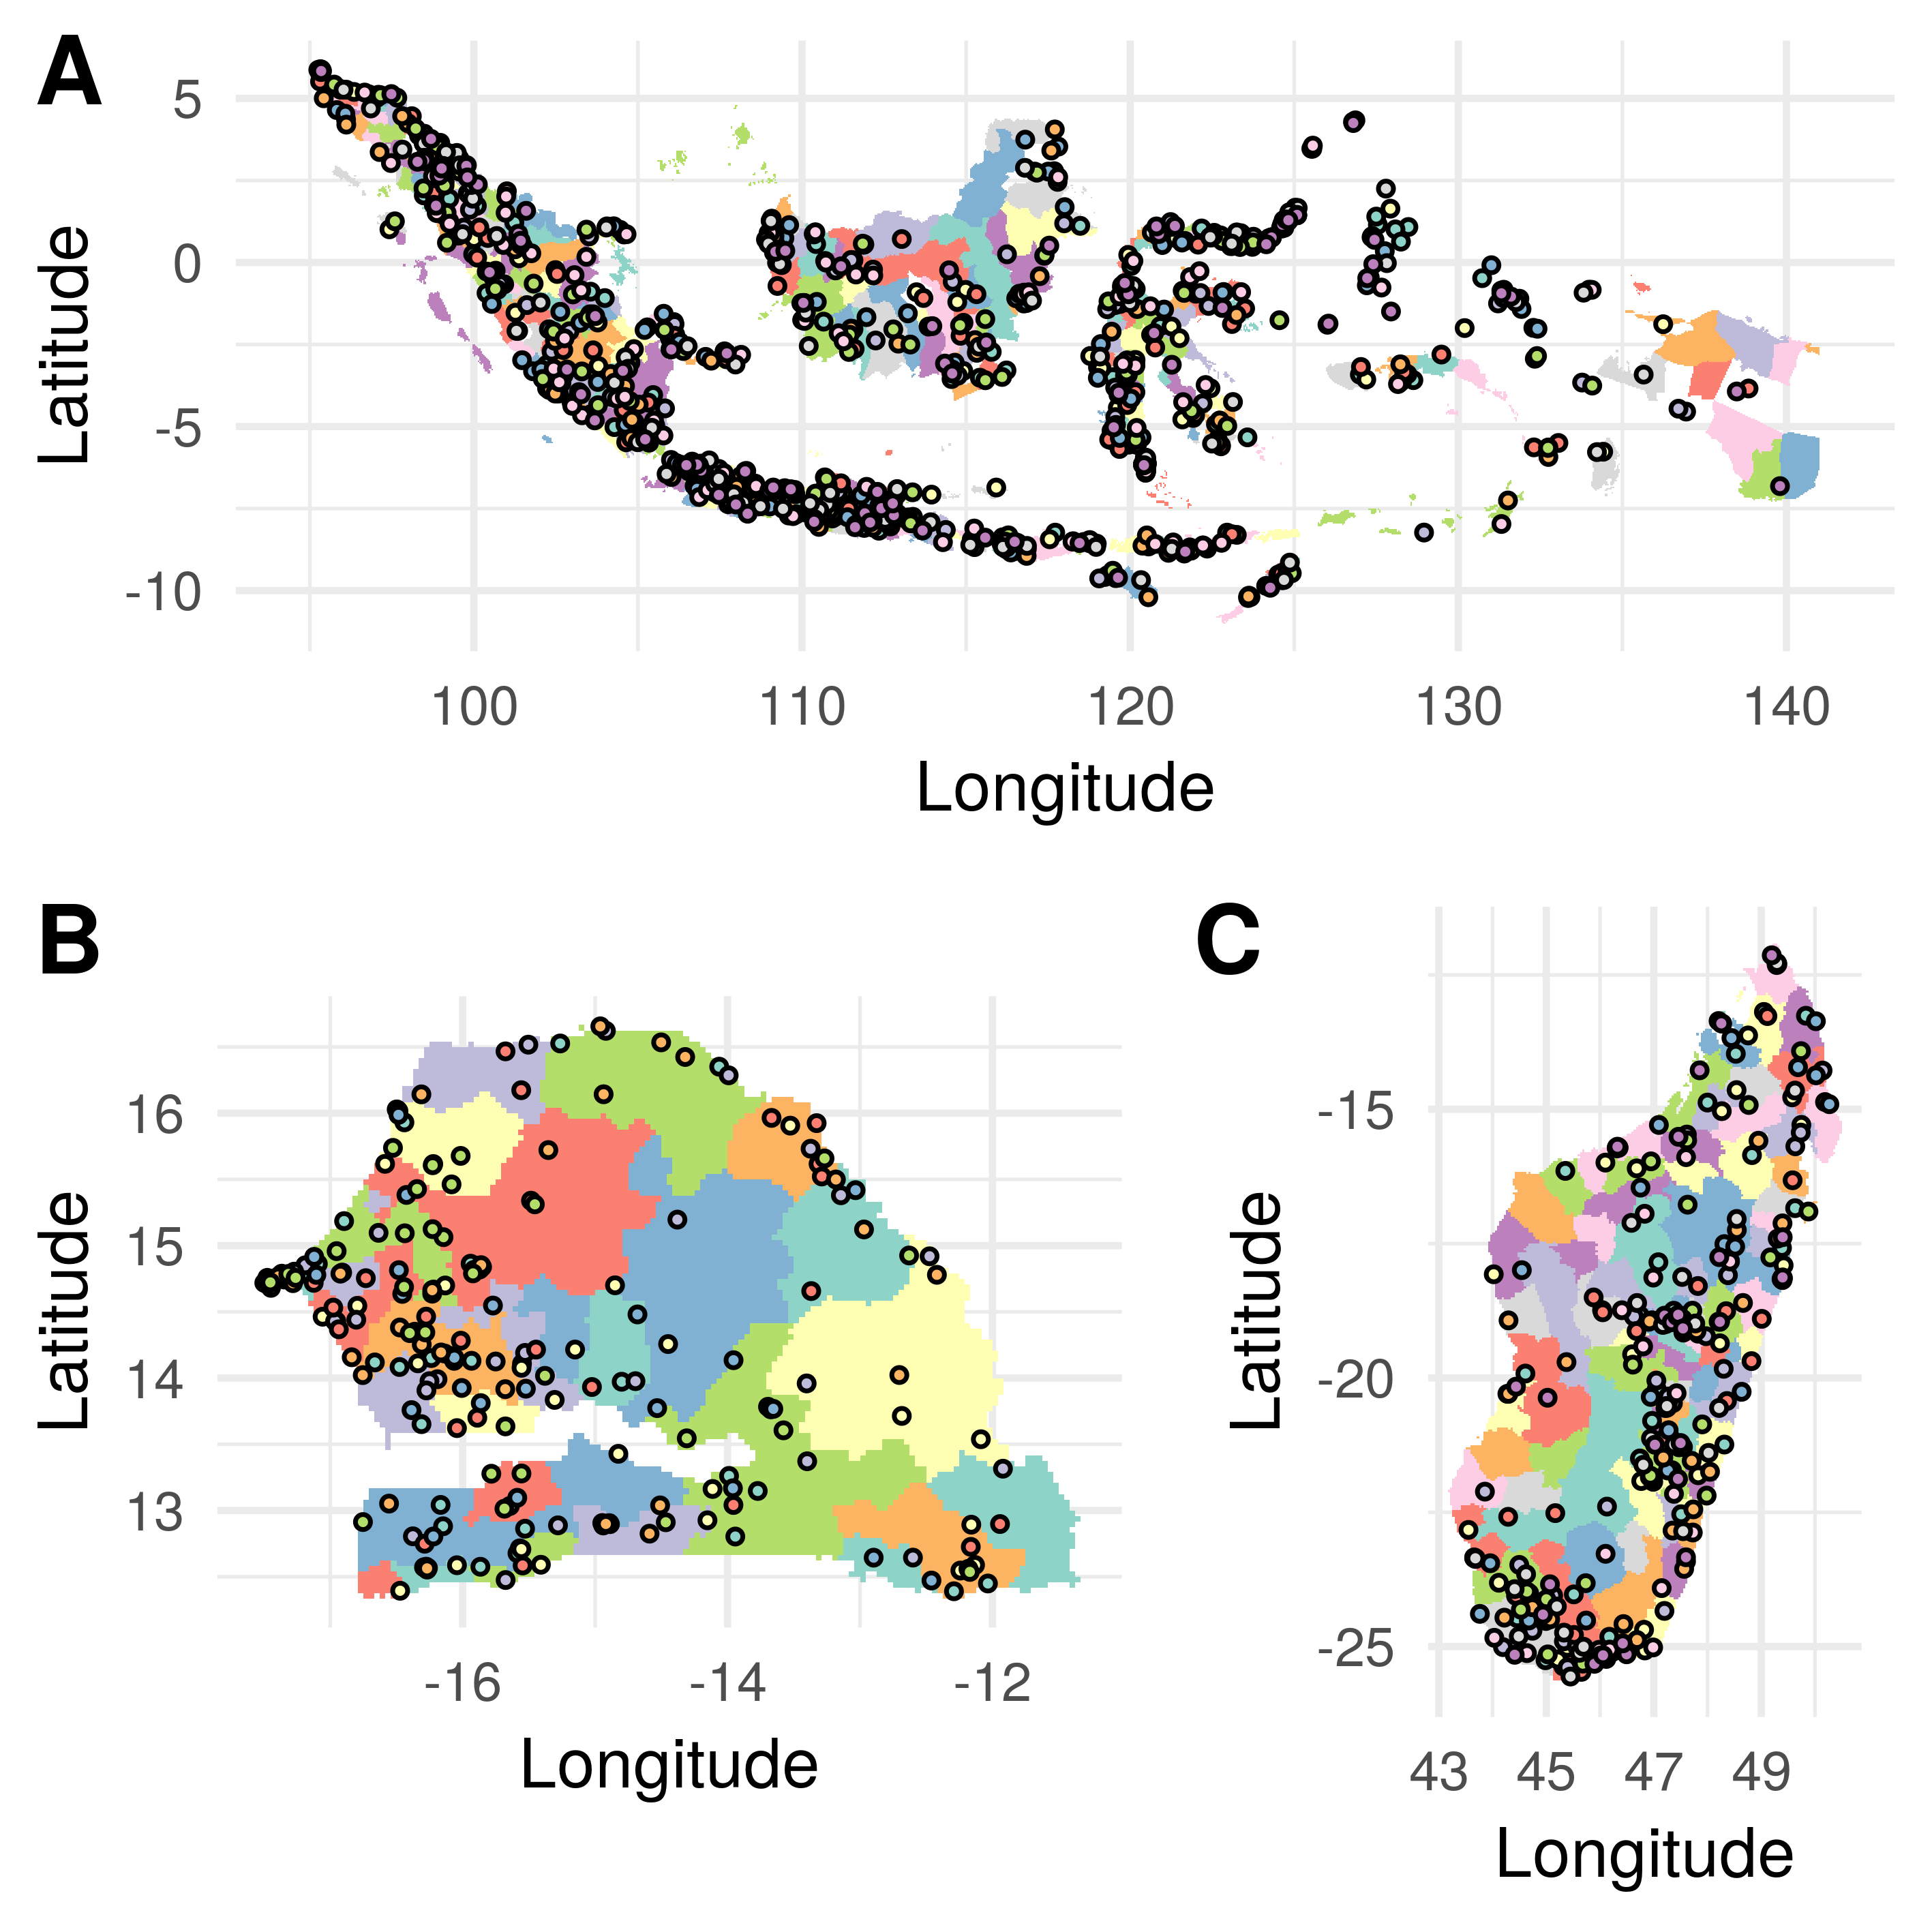
\includegraphics[width = 0.9\textwidth]{figures/random_crossvalidation_full.png} %\caption{Indonesia random crossvalidation} 

\caption{{\bf Random cross-validation scheme for Indonesia, PseudoSenegal and Madagascar.} The fold for both aggregated incidence data and prevalence point data is shown.}
\label{fig:cv_random}
\end{figure}


\begin{figure}[!t]
% to be removed before submission
\centering

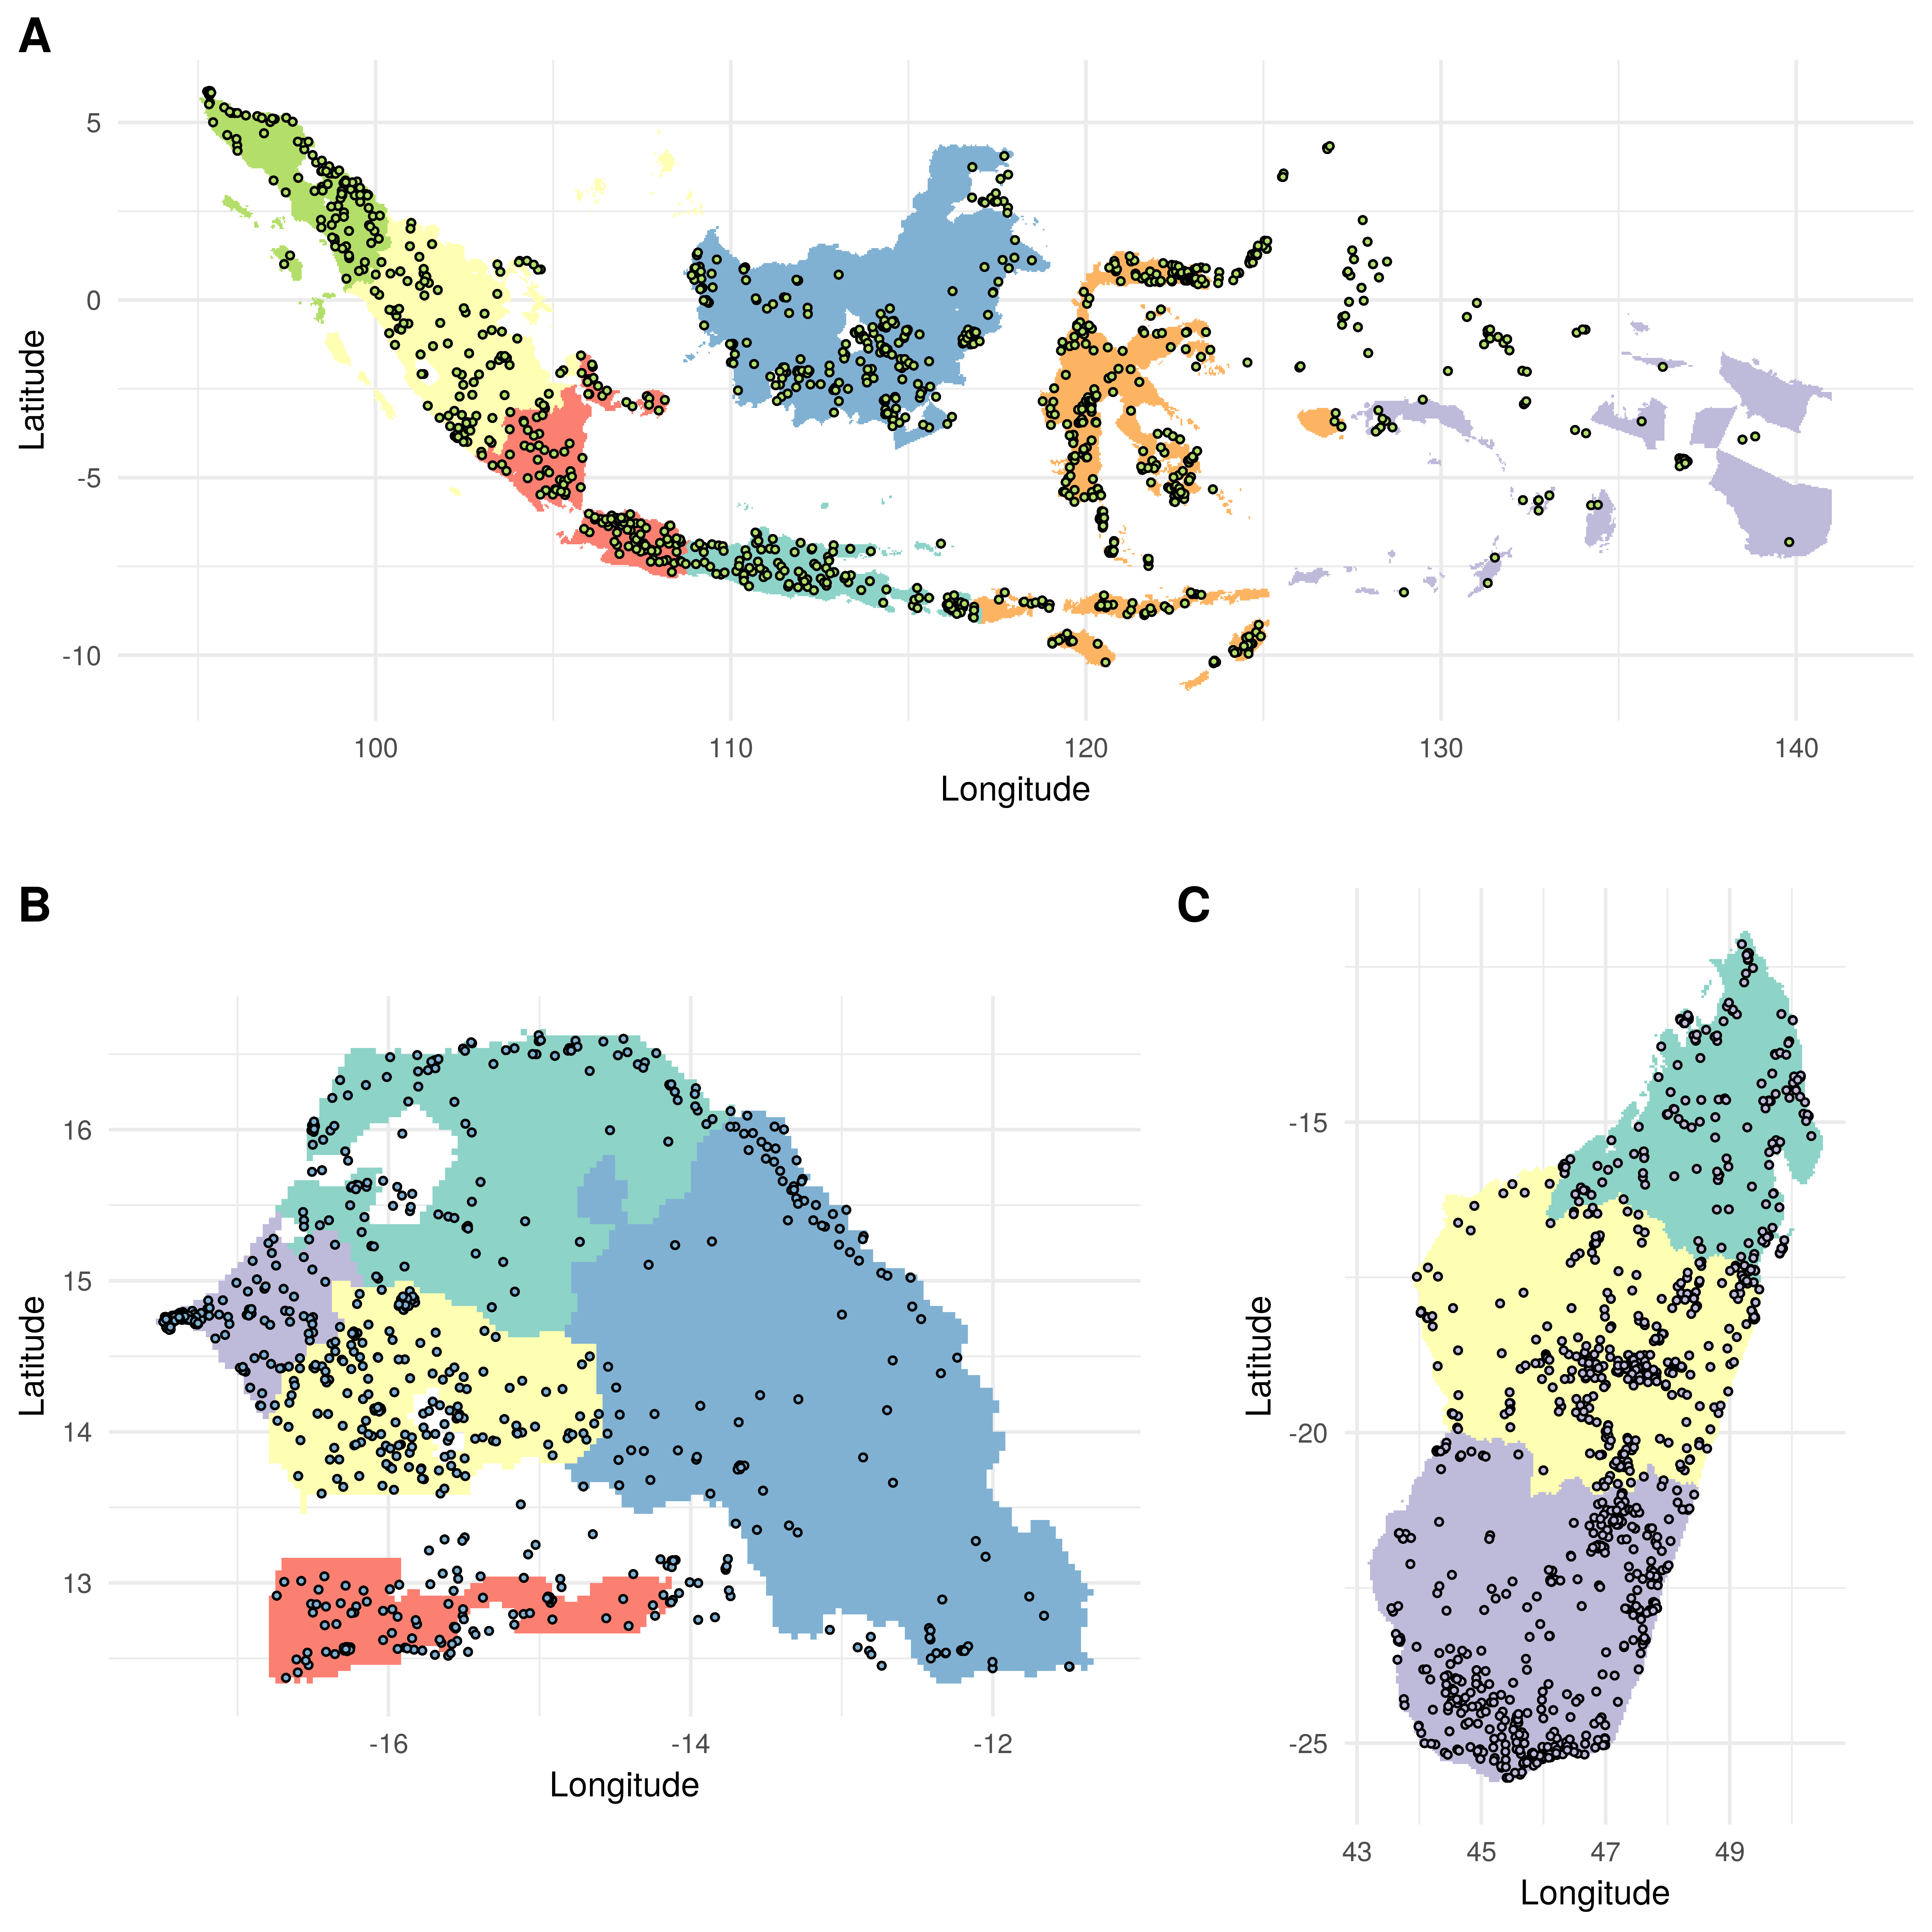
\includegraphics[width = 0.9\textwidth]{figures/spatial_crossvalidation_full.png} %\caption{Indonesia random crossvalidation} 

\caption{{\bf Spatial cross-validation scheme for Indonesia, PseudoSenegal and Madagascar.} The fold for both aggregated incidence data and prevalence point data is shown.}
\label{fig:cv_spatial}
\end{figure}


Finally, we set regularising priors on the regression coefficients $\beta_i \sim \operatorname{Norm}(0, 0.04)$. 
Given the standardised covariates, a regression coefficient from the 95\% IQR of this distribution, and an intercept of -3, each covariate would be able to predict prevalences between 0.004 and 0.27. 
This prior encodes our belief that the full range of malaria transmission can not be explained by a single covariate and our desire to regularise our model.
This regularisation is particularly important given the small number of observations in PseudoSenegal (n = 46) and Madagascar (n = 110).



\subsection*{Experiments}

To compare the three models we used two cross-validation schemes. 
In the first, the combined data set of prevalence and incidence data was split into ten cross-validation folds stratified by data type (Figure~\ref{fig:cv_random}).
This reflects real world data where we in some locations we have incidence data but no prevalence data and visa versa.
Thus this cross-validation scheme can be seen as asking whether the joint model is preferable to using just polygon incidence data.

%figure 1.cross validation. %% Do fig 1 and 2, random and spatial cv. IDN on top, MDG and SEN below in each.


In the second validation scheme the data was split into spatial cross-validation folds (see Figure~\ref{fig:cv_spatial}).
The number of folds was seven for Indonesia, four for PseudoSenegal and three for Madagascar due to their differing sizes and geographies.
The data was divided by combining the prevalence point-survey locations and the centroids of the incidence polygons and performing k means clustering.
This scheme is testing the models' ability to predict into new areas with little information from the spatial random field.

In both cases we examined performance metrics for both the withheld prevalence point-survey data and the withheld incidence polygon data.
As there is no good way of combining predictive error from both types of data into one performance metric, we considered performance separately throughout.
We considered the ability to predict polygon incidence correctly our main objective and our performance metric was mean absolute error (MAE).
However, a problem with using polygon data in a cross-validation scheme is that a model can perform well at the polygon level but not correctly predict the pixel-level malaria risk.
Predictive performance on prevalence survey-points is one way to measure how well a model can predict pixel-level malaria risk.
However, in areas of low prevalence, small or moderately sized prevalence point-surveys can be noisy or unsensitive and so care must be taken when interpreting predictive performance on these data.
Therefore our secondary metric was MAE, weighted by survey sample size, of prevalence point-surveys.
While other metrics could have been used, we specifically did not use correlation as correlation measures linear dependance without regard to slope or intercept.
As the models are being fitted on data on difference scales we found that observations and predictions were sometimes correlated but strongly displaced from the one-one line and therefore correlation metrics were misleading.
% Why not correlation
To assess how well the models were calibrated we considered coverage of the 80\% predictive credible intervals on the hold-out data.




\begin{table}[!t]
\begin{adjustwidth}{-2.25in}{0in} % Comment out/remove adjustwidth environment if table fits in text column.
\centering
\caption{
{\bf Summary of out-of-sample accuracy for random cross-validation experiment.}}
\begin{tabular}{llllll}
\hline
{\bf Holdout data} & {\bf Country} &  {\bf Points} & {\bf Polygons} & {\bf Joint} \\
\thickhline 
Incidence & Indonesia & 18.33 & {\bf 14.02} &  14.09\\
& PseudoSenegal & 51.24 & {\bf 26.74} &  28.45\\
& Madagascar & 85.54 & 37.45 &  {\bf 34.49}\vspace{3mm}\\
Prevalence & Indonesia & 0.010 & 0.010 &  0.010\\
& PseudoSenegal & {\bf 0.015} & 0.024 &  0.024\\
& Madagascar & {\bf 0.054} & 0.059 &  0.059\\
\end{tabular}
\begin{flushleft}
Mean absolute error of predicted incidence rate and weighted mean absolute error of prevalence against out-of-sample observed data for three countries.
The data were split randomly into 10 groups stratified by data type (incidence polygon and prevalence points).
\end{flushleft}
\label{table1}
\end{adjustwidth}
\end{table}


\begin{table}[!t]
\begin{adjustwidth}{-2.25in}{0in} % Comment out/remove adjustwidth environment if table fits in text column.
\centering
\caption{
{\bf Summary of out-of-sample accuracy for spatial cross-validation experiment.}}
\begin{tabular}{llllll}
\hline
{\bf Holdout data} & {\bf Country} &  {\bf Points} & {\bf Polygons} & {\bf Joint} \\
\thickhline 
Incidence & Indonesia &  18.13 &  {\bf 14.77} &   15.02\\
& PseudoSenegal &  51.17 &  41.43 &   {\bf 36.76}\\
& Madagascar & 107.32 &  71.44 &   {\bf 65.50}\vspace{3mm}\\
Prevalence & Indonesia & 0.011 & {\bf 0.010} &  {\bf 0.010}\\
& PseudoSenegal & {\bf 0.015} & 0.019 &  0.019\\
& Madagascar & 0.069 & 0.066 &  {\bf 0.065}\\
\end{tabular}
\begin{flushleft}
Mean absolute error of predicted incidence rate and weighted mean absolute error of prevalence against out-of-sample observed data for three countries.
The data were split into seven, four and three groups in Indonesia, PseudoSenegal and Madagascar respectively.
\end{flushleft}
\label{table2}
\end{adjustwidth}
\end{table}



% Results and Discussion can be combined.
%%%%%%%%%%%%%%%%%%%%%%%%%%%%%%%%%%%%%%%%%%%%%%%%%%%%%%%%%%%%%%%%%%%%%%%%%%%%%%%%%%%%%%%%%%%%%%%%%%%%%
\section*{Results}
%%%%%%%%%%%%%%%%%%%%%%%%%%%%%%%%%%%%%%%%%%%%%%%%%%%%%%%%%%%%%%%%%%%%%%%%%%%%%%%%%%%%%%%%%%%%%%%%%%%%%



% Random results
% Maps, reasonable for both
% MAE performance.

For the random cross-validation experiments, the polygon-only model had the lowest mean absolute error, with respect to predicting incidence, for Indonesia and PseudoSenegal (Table~\ref{table1}).
Incidence in Madagascar was best predicted by the joint model.
However, the difference between the two models in Indonesia was small.
Scatter plots of the out-of-sample predictions can be seen in Figures~\ref{randompredobsscatter}A, C and E.
From the scatter plots it can be seen that the point-only model is strongly biased, overestimating incidence in Indonesia and Madagascar and underestimating incidence in Senegal.


%figure 5, 6. Spat and random cv. PR vs Poly columns, countries as rows, model as colour?
\begin{figure}
% to be removed before submission
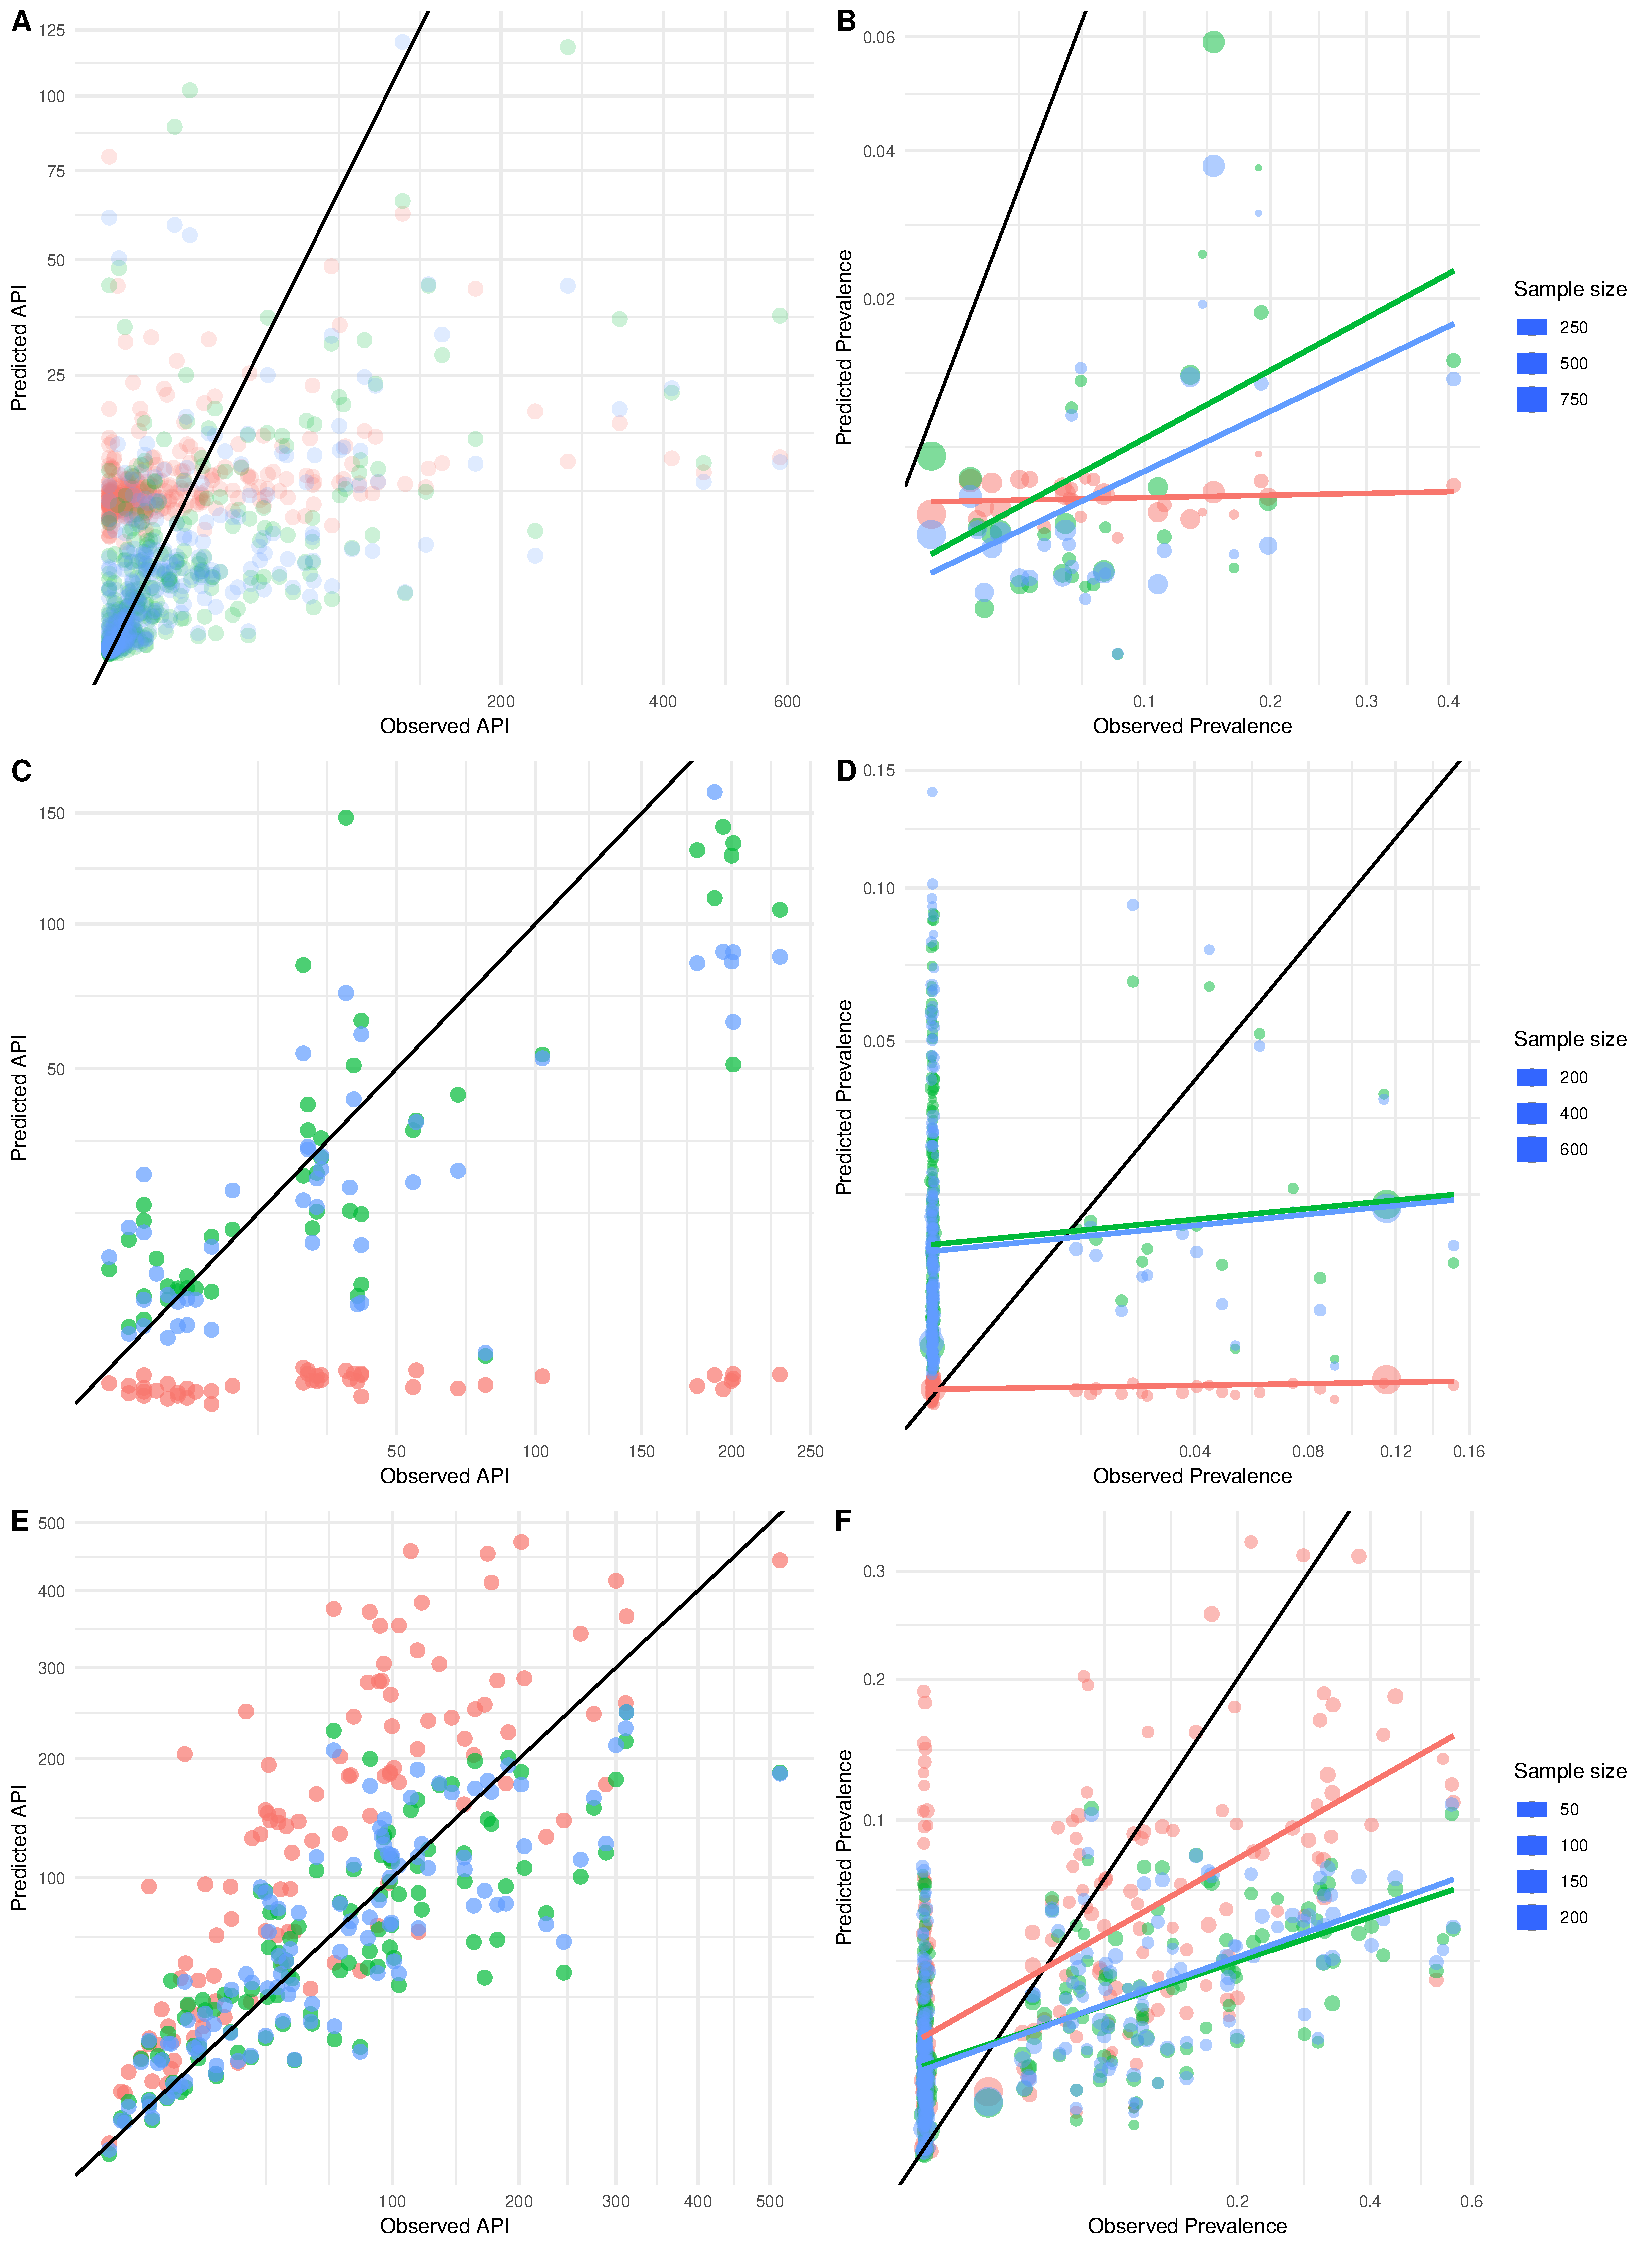
\includegraphics[width = 1.05\textwidth]{figures/random_cv_scatter.pdf} %\caption{Indonesia spatial crossvalidation} 
\caption{{\bf Observed-predicted plots for random cross-validation experiments.}
A-B) Indonesia, C-D) PseudoSenegal, E-F) Madagascar. A, C, E) square root aggregated incidence (per 1,000), B, D, F) square root prevalence.
Results from all three models are included with the points only model being shown in orange, the downscaling model being shown in blue and the combined model being shown in green.
The bimodal distribution in observed prevalence in Indonesia is caused by the large number of surveys with exactly one positive case.
}
\label{randompredobsscatter}
\end{figure}





%figure 5, 6. Spat and random cv. PR vs Poly columns, countries as rows, model as colour?
\begin{figure}
% to be removed before submission
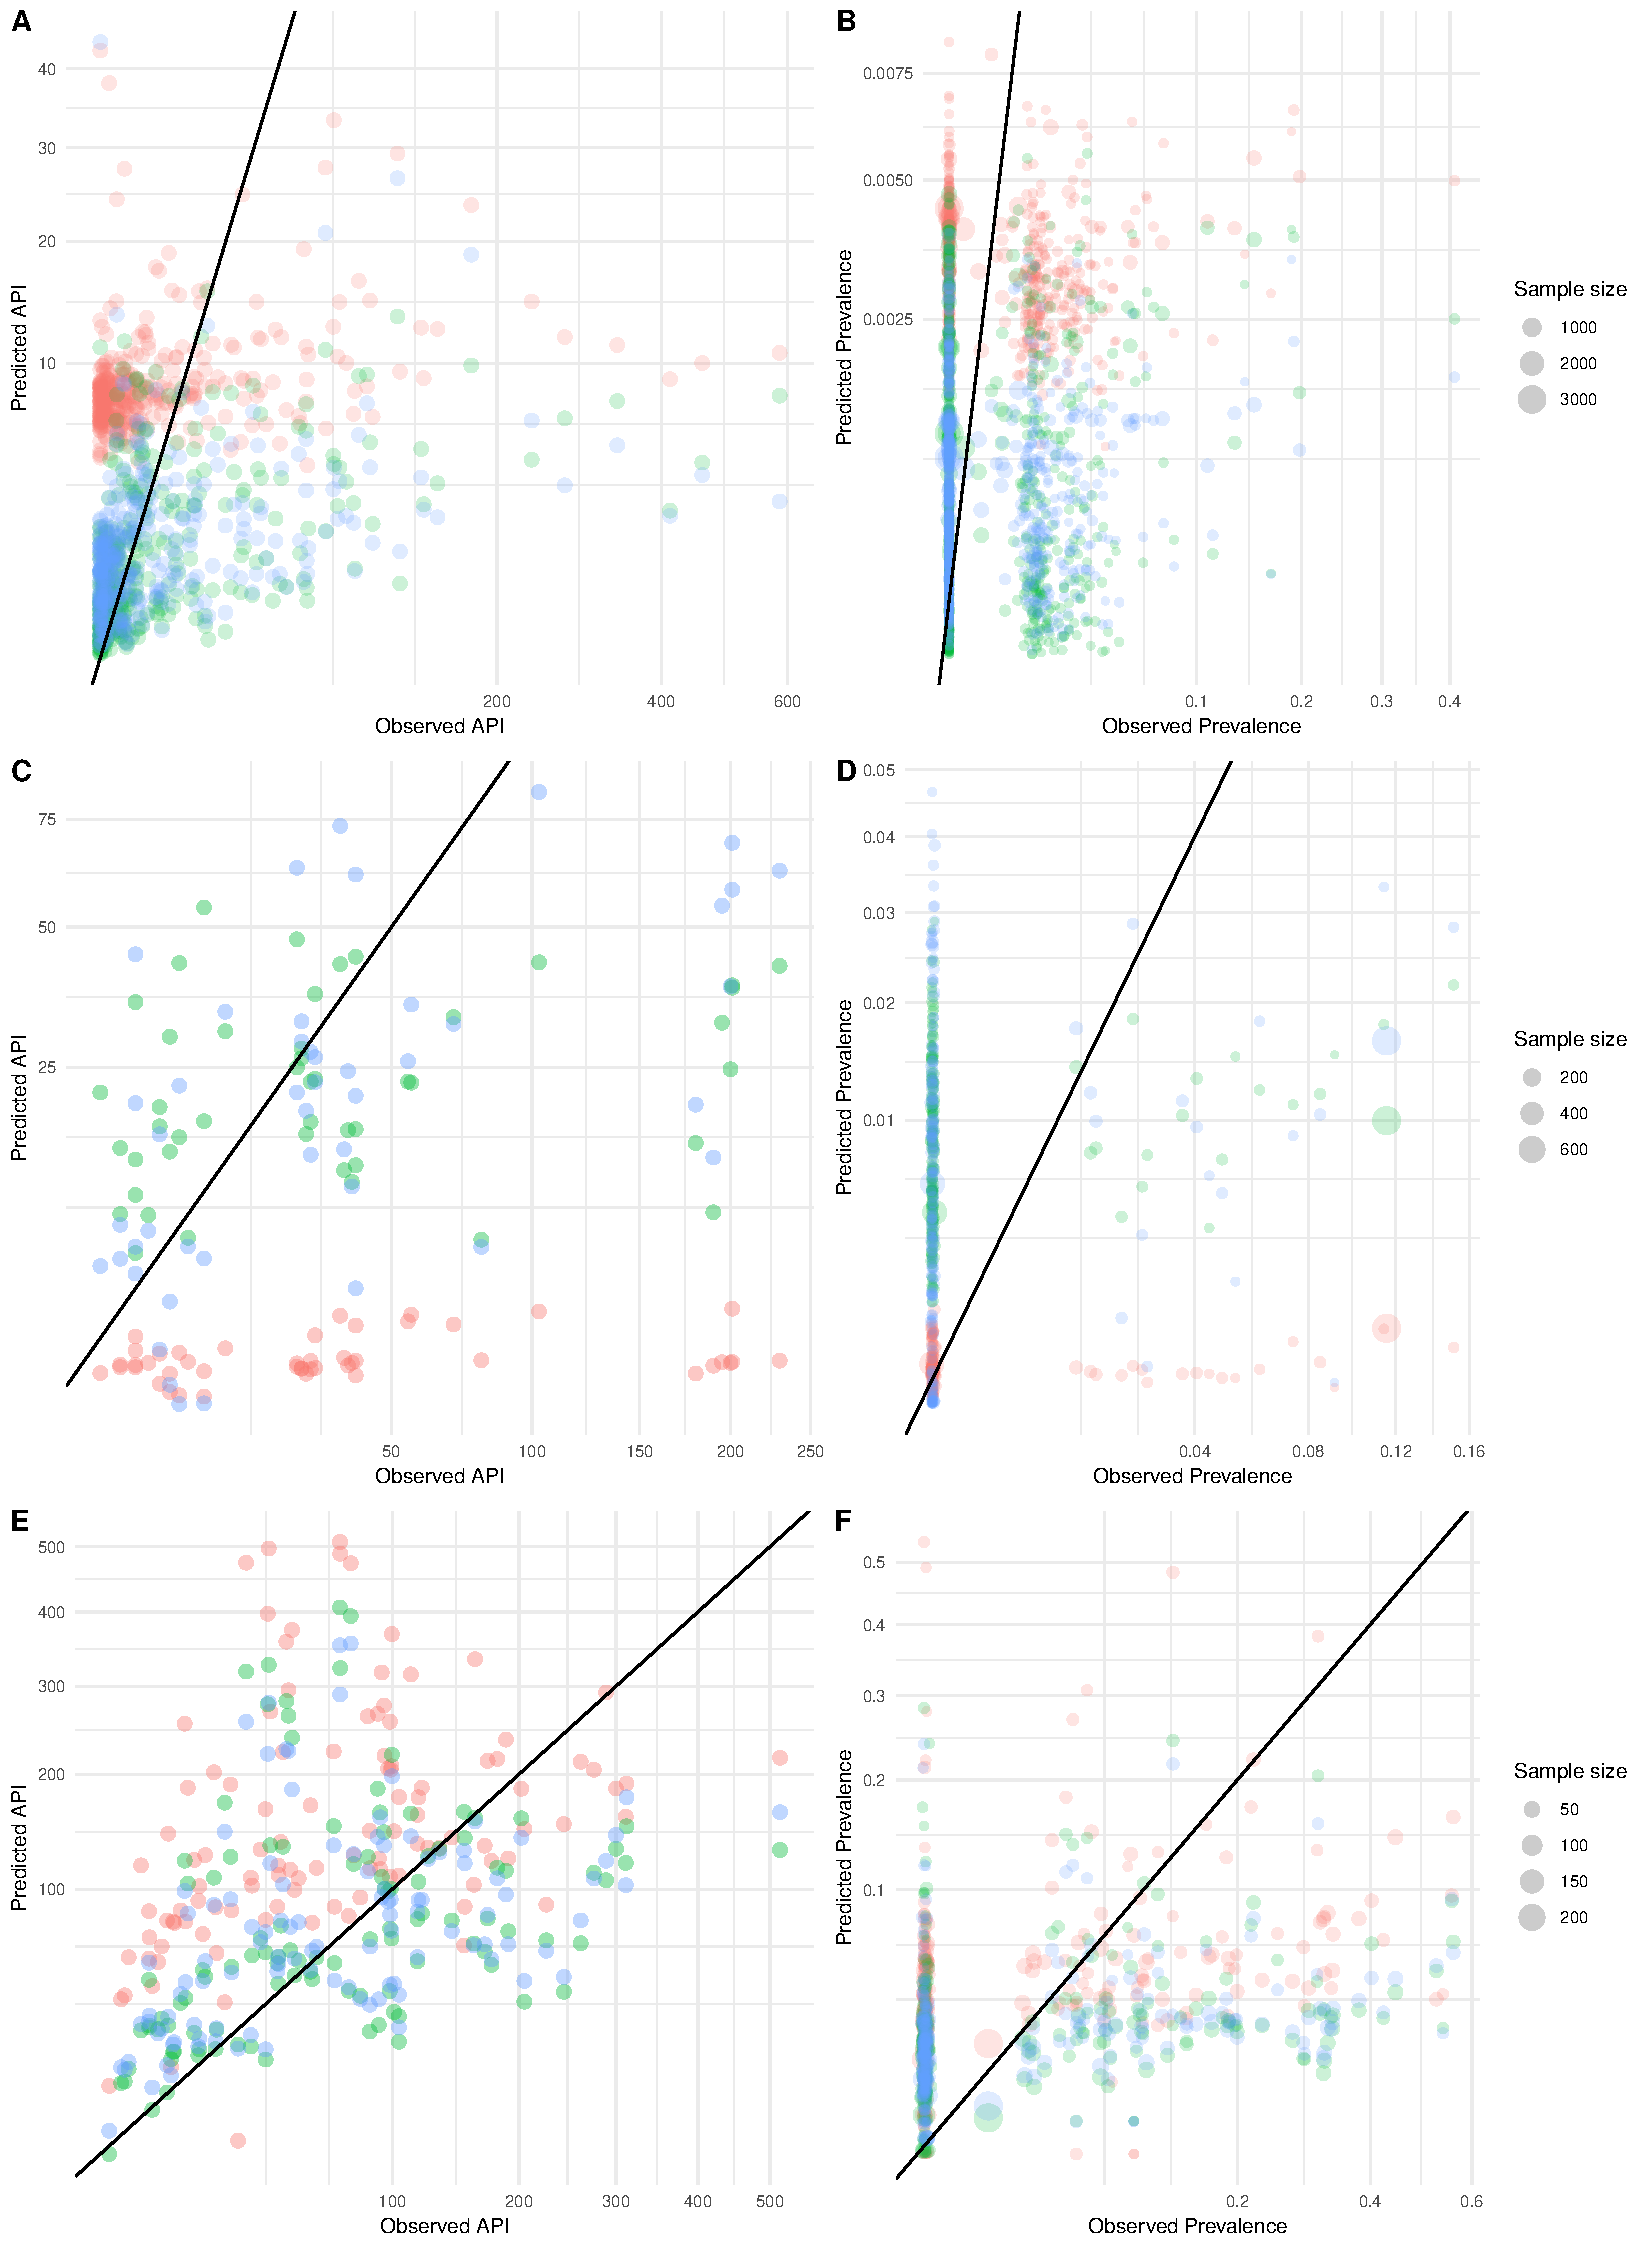
\includegraphics[width = 1.05\textwidth]{figures/spatial_cv_scatter.pdf} %\caption{Indonesia spatial crossvalidation} 
\caption{{\bf Observed-predicted plots for spatial cross-validation experiments.}
A-B) Indonesia, C-D) PseudoSenegal, E-F) Madagascar. A, C, E) square root aggregated incidence (per 1,000), B, D, F) square root prevalence.
Results from all three models are included with the points only model being shown in orange, the downscaling model being shown in blue and the combined model being shown in green.
The bimodal distribution in observed prevalence in Indonesia is caused by the large number of surveys with exactly one positive case.
}
\label{spatialpredobsscatter}
\end{figure}


\begin{table}[t]
\begin{adjustwidth}{-2.25in}{0in} % Comment out/remove adjustwidth environment if table fits in text column.
\centering
\caption{
{\bf Summary of coverage of 80\% credible intervals.}}
\begin{tabular}{llllll}
\hline
{\bf Holdout data} & {\bf Cross-validation} & {\bf Country} &  {\bf Points} & {\bf Polygons} & {\bf Joint} \\
\thickhline 
Incidence & Random & Indonesia & 0.13 & 0.72 &  0.73\\
&& PseudoSenegal & 0.11 & 0.80 &  0.85\\
&& Madagascar & 0.59 & 0.82 &  0.77\vspace{1mm}\\
& Spatial & Indonesia & 0.14 & 0.76 &  0.68\\
&& PseudoSenegal & 0.30 & 0.67 &  0.70\\
&& Madagascar & 0.68 & 0.65 &  0.68\vspace{3mm} \\
Prevalence & Random & Indonesia & 0.90 & 0.50 &  0.80\\
&& PseudoSenegal & 0.80 & 0.71 &  0.91\\
&& Madagascar & 0.83 & 0.53 &  0.74\vspace{1mm}\\
& Spatial & Indonesia & 0.87 & 0.62 &  0.96\\
&& PseudoSenegal & 0.90 & 0.88 &  0.79\\
&& Madagascar & 0.93 & 0.68 &  0.83\\
\end{tabular}
\begin{flushleft}

\end{flushleft}
\label{table3}
\end{adjustwidth}
\end{table}


The benchmark points-only model had the lowest weighted MAE between observed and predicted prevalence for both PseudoSenegal and  Madagascar while the wighted MAE was the same for all three models in Indonesia (Table~\ref{table1}).
The more pertinent comparison is whether the addition of the prevalence data improves the ability of the polygon-only models to predict pixel level prevalence.
However, weighted MAE was unchanged between the polygon-only model and the joint model for Indonesia, PseudoSenegal or Madagascar.
Scatter plots of the out-of-sample predictions can be seen in Figures~\ref{randompredobsscatter} B, D and F.
All models show poor predictive performance in Indonesia and PseudoSenegal with none of the models being able to accurately predict the large number of points with zero prevalence.
The predictions in Madagascar are better though the large number of surveys with measured prevalence of zero are still problematic. 

Maps of the Indonesian input data and predictions (Figures~\ref{predobsmapidn}A and B) indicate that the broad spatial patterns of malaria incidence were recovered with areas in Papua, Borneo and Suluwasi being estimated as relatively high risk.
Similarly, input data and predictions (Figures~\ref{predobsmapsen}A and B) for PseudoSenegal show broad agreement with malaria incidence being higher in the South.


% Further results. Accuracy or recall of Sen. Correlation for some?

% Spatial results
% Maps, reasonable for india, get's broad pattern even far away from data. Poor for SEN, wrong overall pattern. Different covariates.
% MAE performance.

For the spatial cross-validation experiments, the joint model had the best predictive performance for both PseudoSenegal and Madagascar.
The polygon-only model again had the lowest mean absolute error between observed and predicted incidence for Indonesia (Table~\ref{table2}).
Scatter plots of the out-of-sample predictions can be seen in Figures~\ref{spatialpredobsscatter}A, C and E.

Again, the benchmark points-only model had the lowest weighted MAE between spatially cross-validated observed and predicted prevalence for PseudoSenegal.
However, for Indonesia, both the polygon-model and the joint model marginally outperformed the points-only model. 
However, scatter plots of the out-of-sample predictions show that there is almost no correlation between observed and predicted values (Figures~\ref{randompredobsscatter} B, D and F).
For PseudoSenegal, the joint model (0.065) had the lowest weighted MAE for predicted prevalence though this was again marginal (points-only 0.069, polygons-only 0.066).
Again the survey-points with prevalence of zero were difficult to correctly predict.

Maps of the Indonesian input data and spatially out-of-sample predictions (Figures~\ref{predobsmapidn}A and C) suggest the that the broad spatial patterns were once again recovered.
This acceptable performance is notable given the very large areas held out-of-sample (Fig~\ref{fig:cv_spatial}).
For example, the whole of Papua and West Papua the the East are held out in a single fold.
In contrast the predictions for PseudoSenegal do not match those observed in the input data (Figures~\ref{predobsmapsen}A and C). 


% Coverage results

The polygon-only model and the joint model seem to be fairly well calibrated (Table~\ref{table3}).
The proportion of out-of-sample incidence datapoints being within their 80\% credible intervals ranged between 0.65 and 0.85.
The proportion of out-of-sample prevalence datapoints being within their 80\% credible intervals ranged from 0.50 to 0.96.
The points-only model was reasonably well calibrated for predictions of prevalence (coverage ranging from 0.8 to 0.93) but was poorly calibrated for predicting incidence with coverage values as low as 0.11 and the best coverage value being 0.68 for spatial cross-validation in Madagascar.

With respect to uncertainty in polygon incidence predictions, the polygon-only model and joint model were similar; adding the prevalence point-survey data sometimes improved coverage and sometimes made it worse.
However, with respect to uncertainty in prevalence point-survey predictions, the coverage was substantially improved in three of six cases and marginally improved in one case.
Coverage improved in the random cross-validation in Indonesia (polygon-only 0.50, joint 0.80) and Madagascar (polygon-only 0.53, joint 0.74) and spatial cross-validation in Madagascar (polygon-only 0.68, joint 0.83) and marginally improved in the spatial cross-validation in PseudoSenegal (polygon-only 0.88, joint 0.79).
In the remaining two cases, adding prevalence point-surveys did not substantially improve coverage, but did make the model more conservative, with coverage of 0.91 rather than 0.71 in the random cross-validation PseudoSenegal experiment and 0.96 instead of 0.62 in the spatial cross-validation Indonesia experiment.

% Overall












%figure 3 and 4. data and predicted incidence maps. Indonesia and PseudoSenegal only. Fig 3 ind, fig 4 rand. Data, Rand, Spatial for best model? Joint model?

\begin{figure}
% to be removed before submission
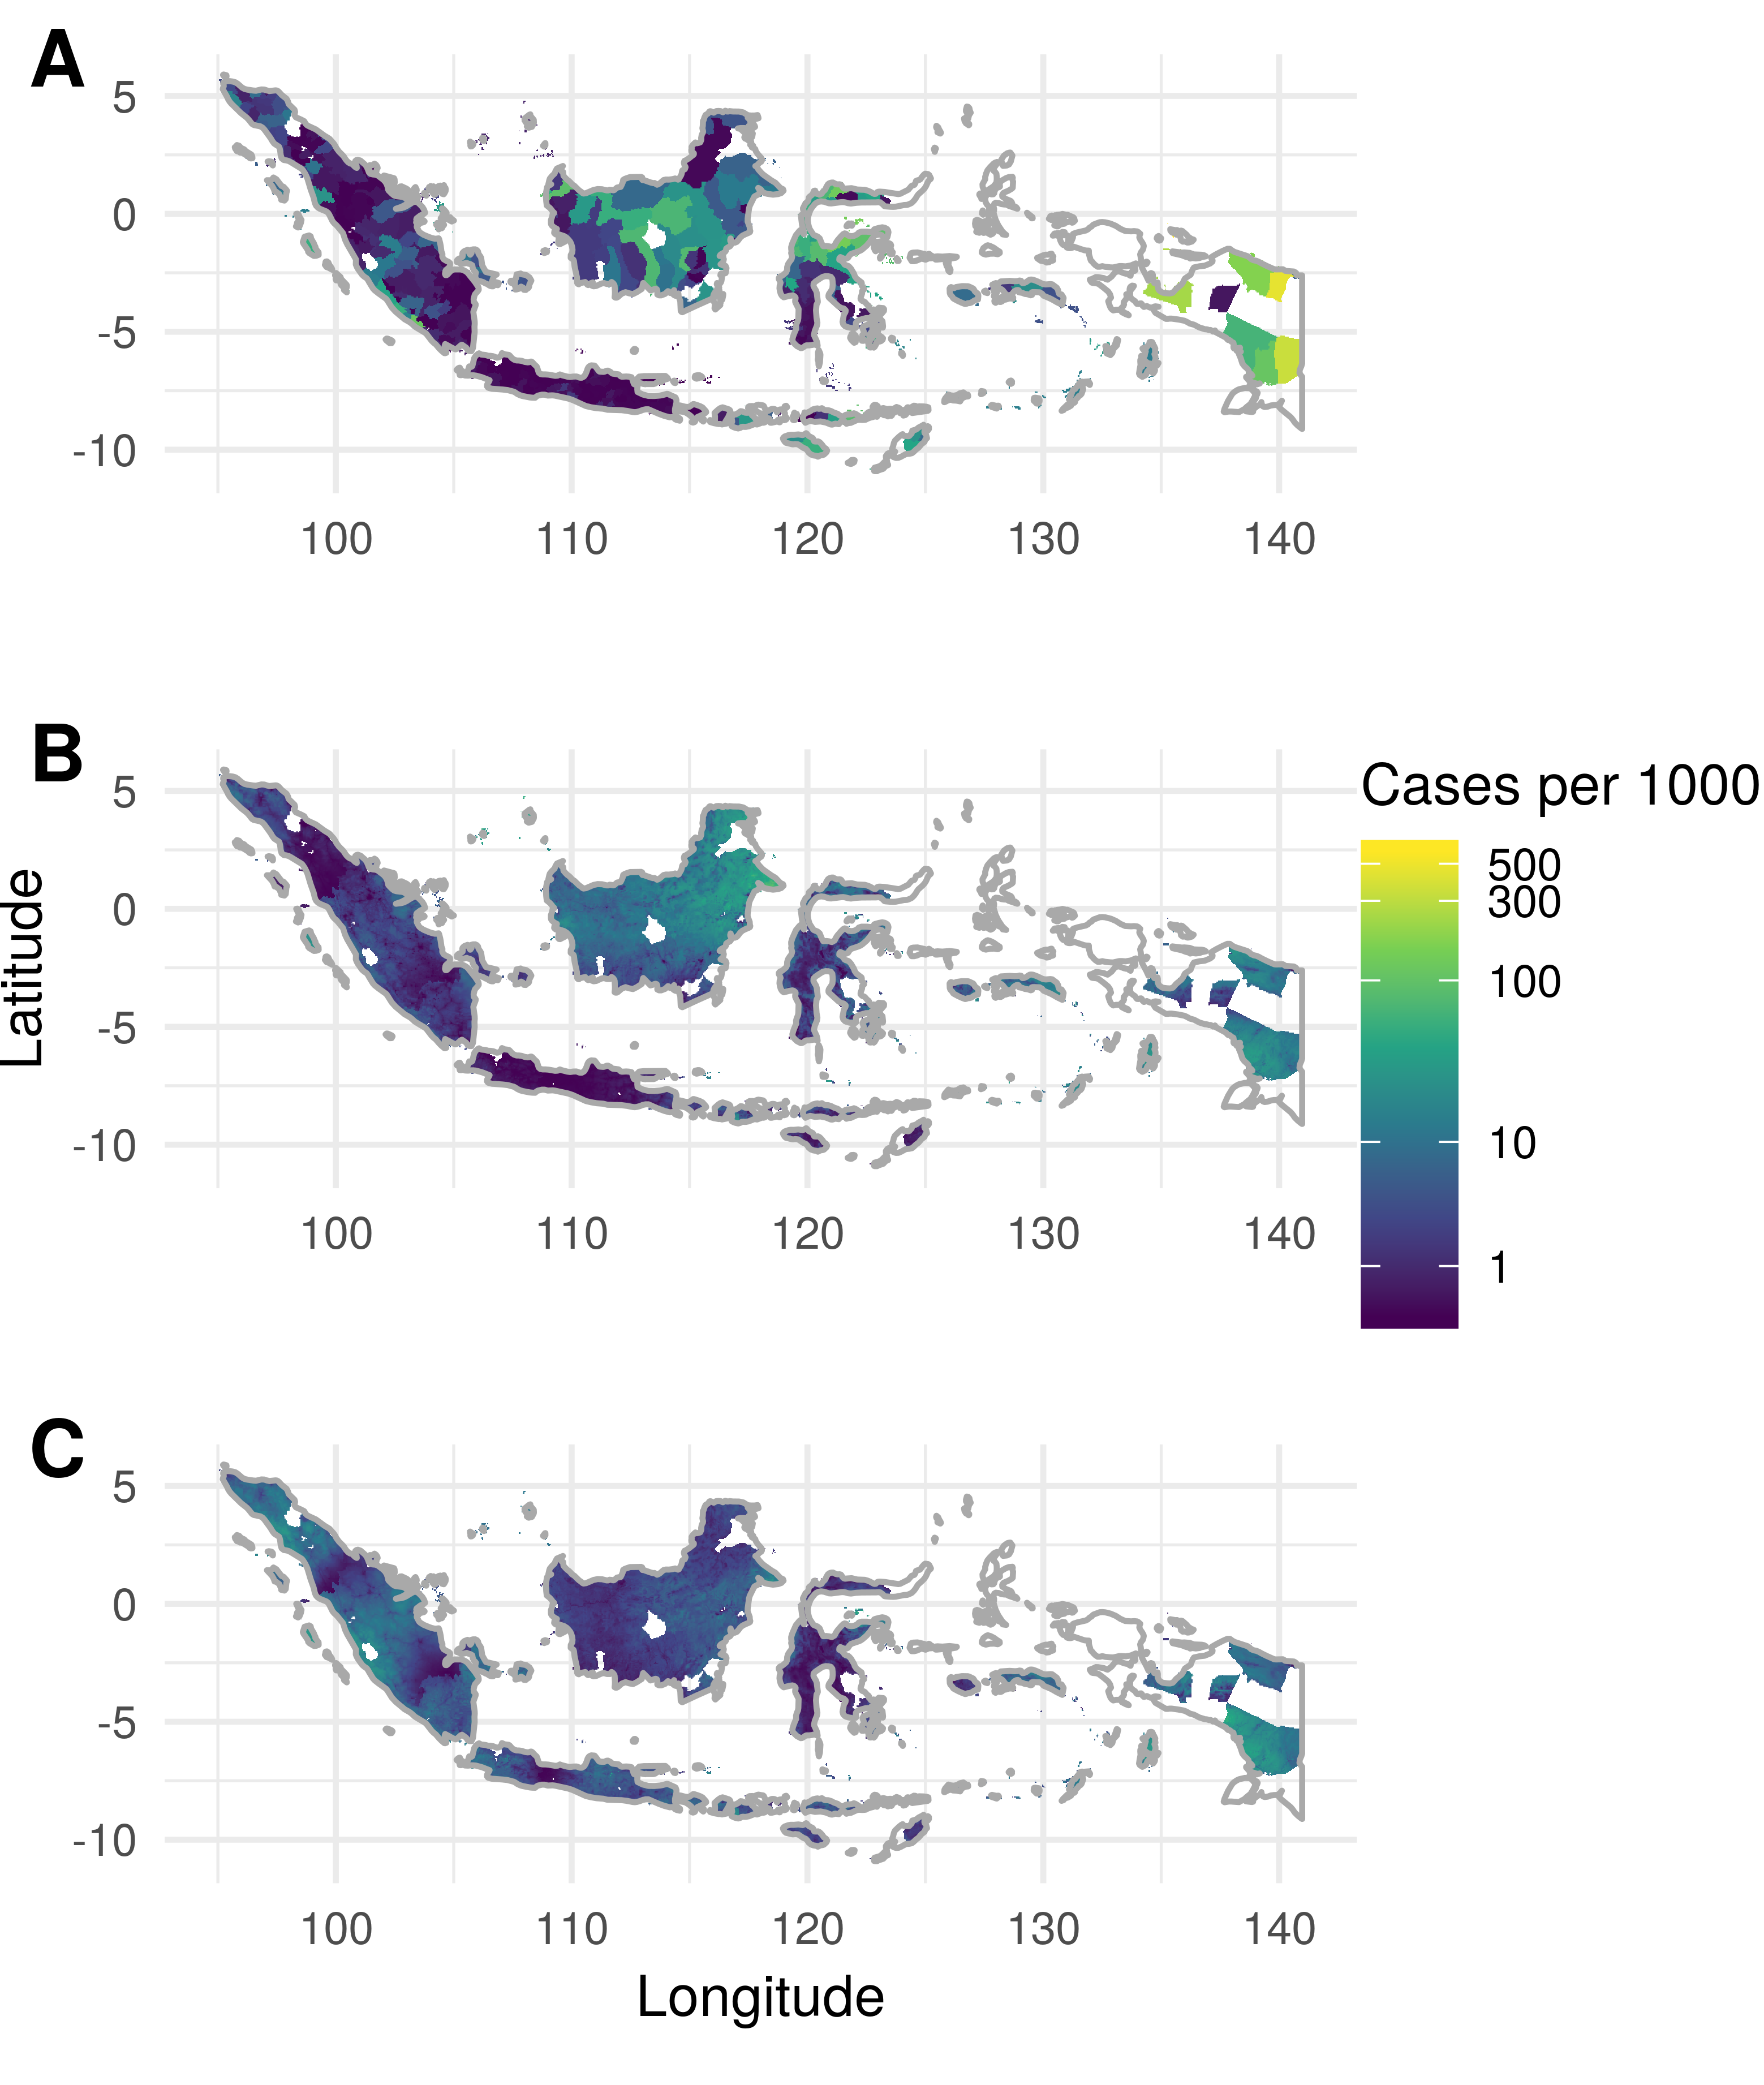
\includegraphics[width = 0.7\textwidth]{figures/idn_both_cv12_preds.png}
\caption{{\bf Input incidence data and predicted incidence maps. } 
The incidence (log10) data (top), predicted log10 incidence from the joint model for randomly sampled out-of-sample polygons (middle) and predicted log10 incidence from the joint model for spatially sampled out-of-sample polygons (bottom) for Indonesia. The values plotted for areas with no polygon data are the means across all cross-validation folds.
}
\label{predobsmapidn}
\end{figure}




\begin{figure}
% to be removed before submission
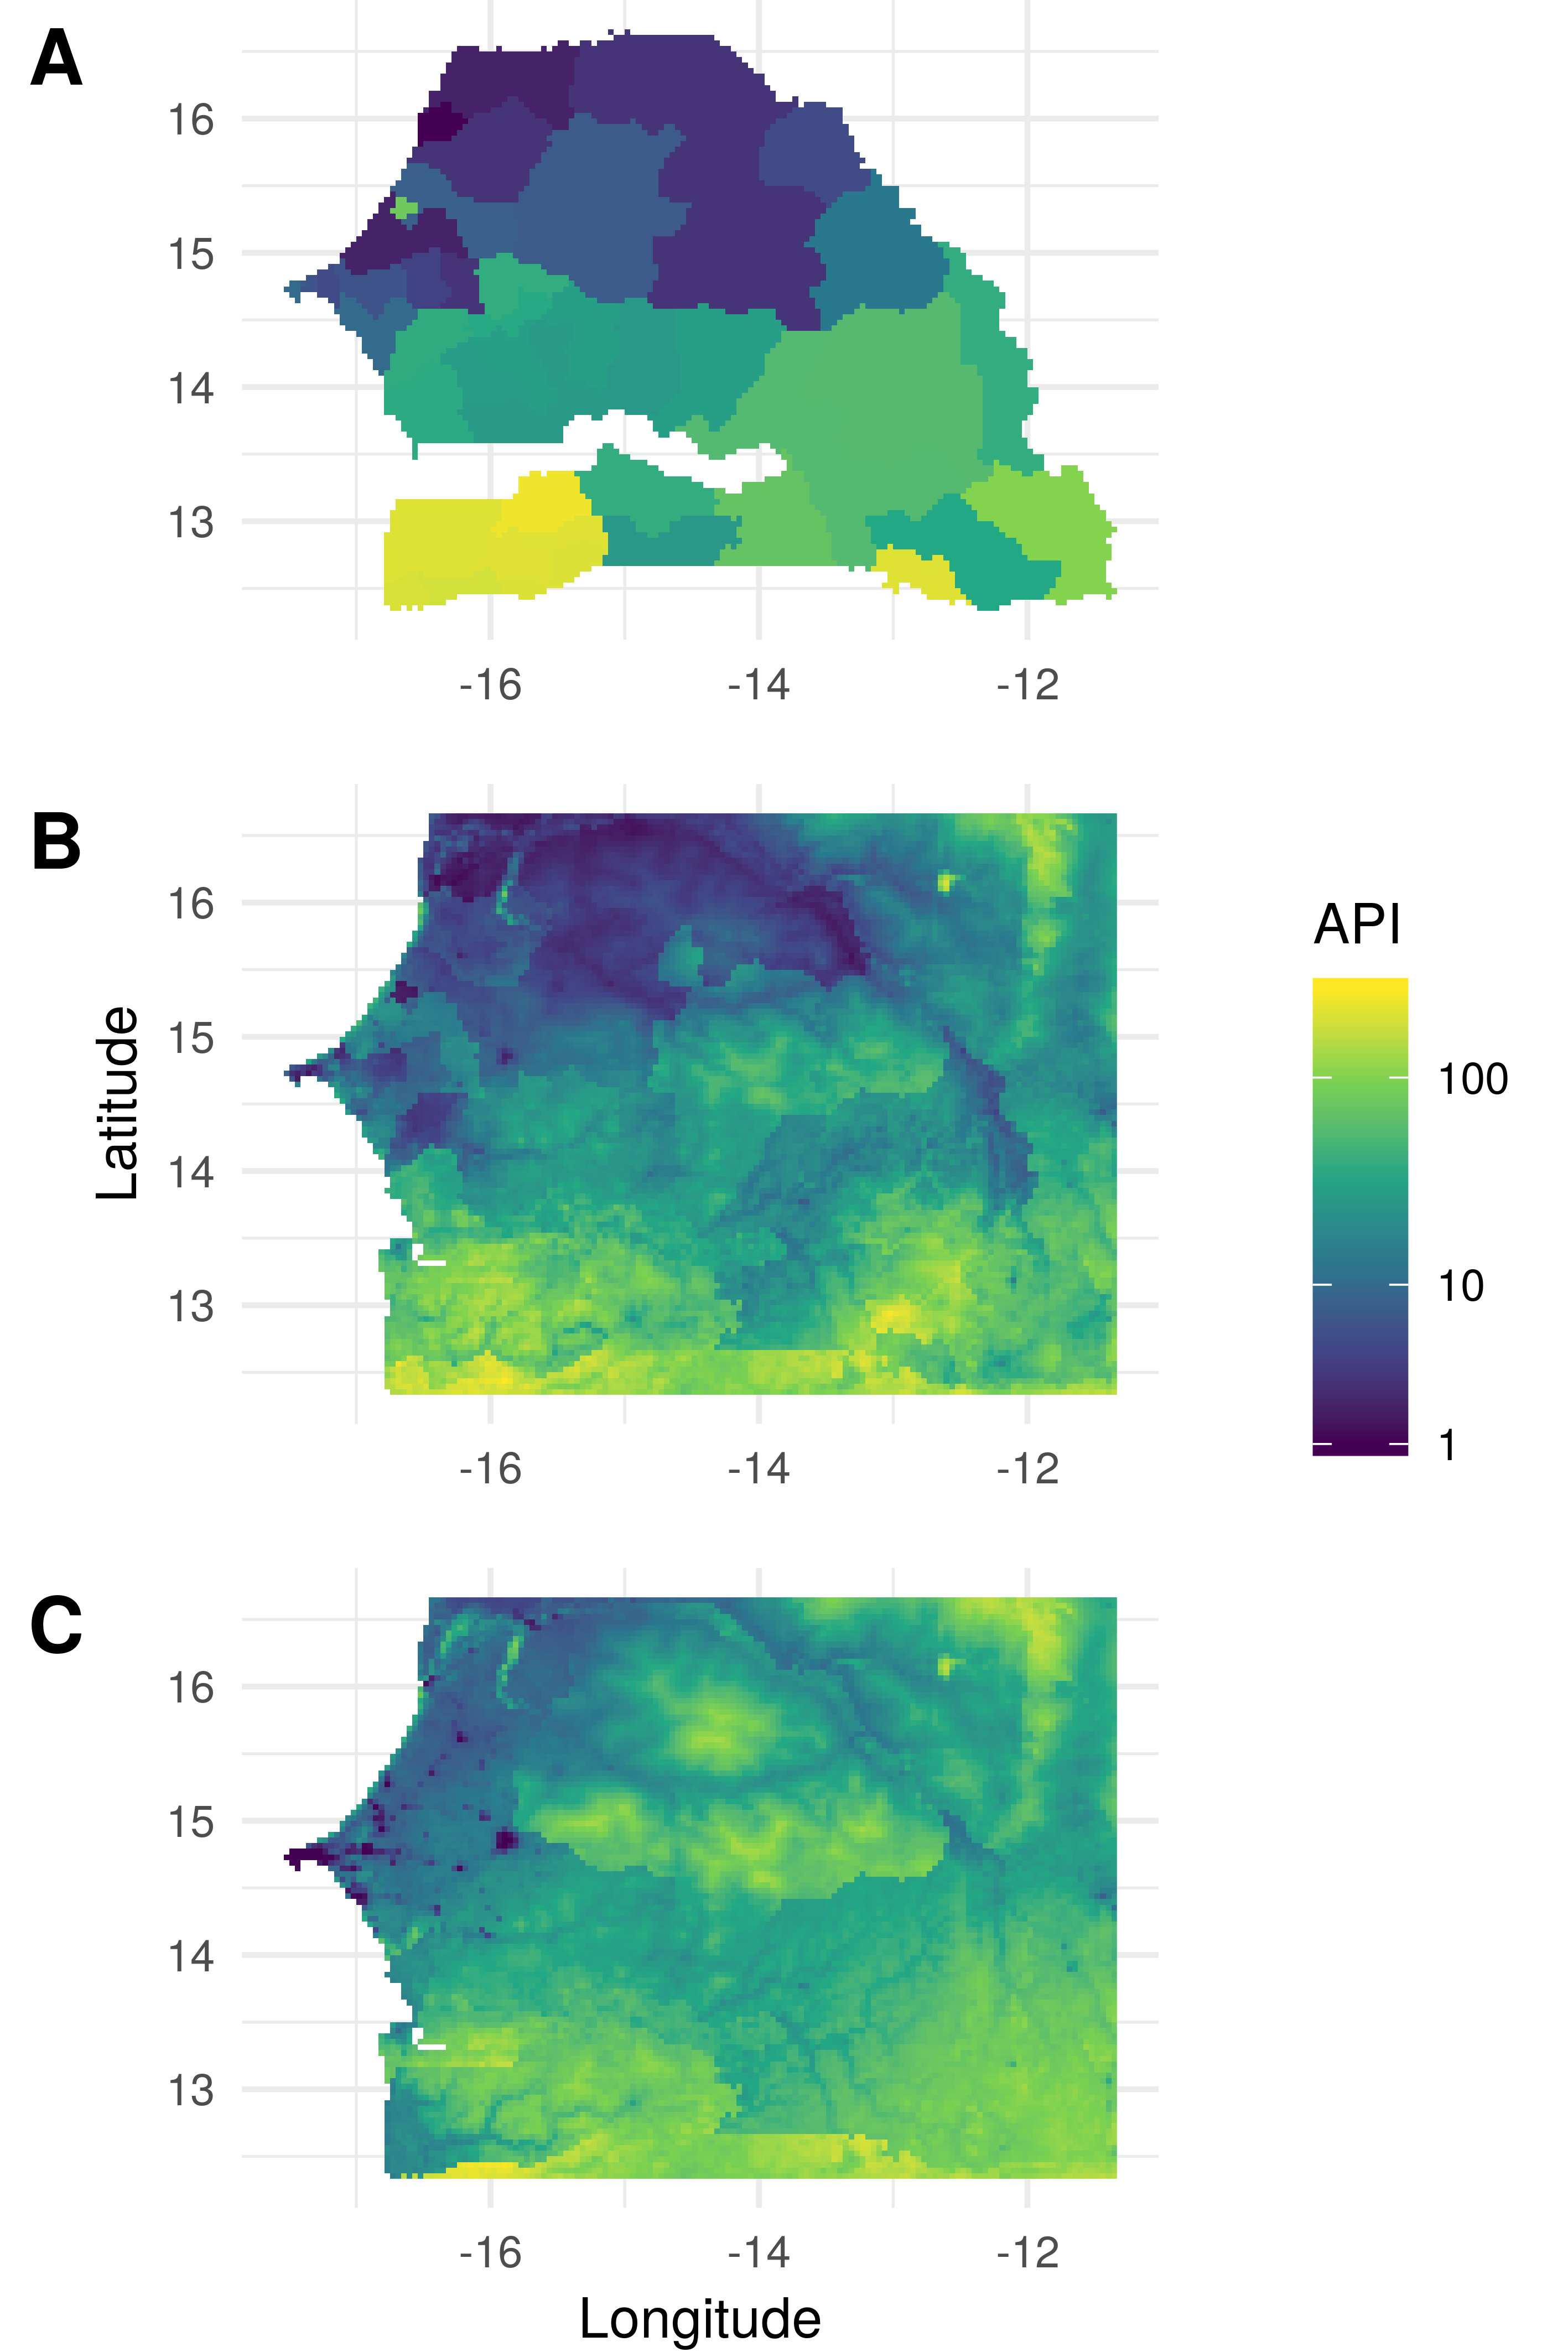
\includegraphics[width = 0.7\textwidth]{figures/sen_both_cv12_preds.png}
\caption{{\bf Input incidence data and predicted incidence maps. } 
The incidence (log10) data, predicted log10 incidence from the joint model for randomly sampled out-of-sample polygons (middle) and predicted log10 incidence from the joint model for spatially sampled out-of-sample polygons (bottom) for PseudoSenegal.
}
\label{predobsmapsen}
\end{figure}


% Results and Discussion can be combined.
%%%%%%%%%%%%%%%%%%%%%%%%%%%%%%%%%%%%%%%%%%%%%%%%%%%%%%%%%%%%%%%%%%%%%%%%%%%%%%%%%%%%%%%%%%%%%%%%%%%%%
\section*{Discussion}
%%%%%%%%%%%%%%%%%%%%%%%%%%%%%%%%%%%%%%%%%%%%%%%%%%%%%%%%%%%%%%%%%%%%%%%%%%%%%%%%%%%%%%%%%%%%%%%%%%%%%


%Summarise results

We have compared the predictive performance of a polygon-only model and a model that jointly learns from polygon incidence data and prevalence point-surveys.
We found that neither model was clearly superior to the other but that both models recovered the broad spatial pattern of malaria risk (Figures \ref{predobsmapidn} and \ref{predobsmapsen}).
With regards to a random cross-validation scheme, adding prevalence point-surveys to the disaggregation model only improved performance in  Madagascar (Table~\ref{table1}).
With regards to a spatial cross-validation scheme, which tests a models ability to predict malaria risk far away from available data, we found that adding the prevalence point-surveys improved on the polygon-only models in both PseudoSenegal and Madagascar but not Indonesia (Table~\ref{table2}).


We used held-out prevalence point-surveys to measure how well model were predicting the within-polygon, pixel-level malaria risk.
Given the poor performance by all models including the points-only model (Figures~\ref{randompredobsscatter} and \ref{spatialpredobsscatter}), particularly in Indonesia and PseudoSenegal these results must be interpreted with care.
% Add sample size, comparisons etc.
In particular, nearly all of the prevalence point-surveys in PseudoSenegal found zero malaria infections (though the age standardisation moves these to slightly non-zero values).
Given the poor performance of the points-only model, it is not useful to interpret these results as a direct measure of a models ability to predict within-polygon, pixel level risk.
Instead we can, with care, interpret the relative performance of models.
In five cases, the polygon-only and joint model had the same predictive performance on the prevalence point-surveys.
In only one cases, the joint model was marginally better.
Therefore we have no evidence that the joint model is better than the polygon-only model at predicting within-polygon, pixel-level malaria risk.




% Discuss and interpret. Generalise


The joint model improved the prediction of polygon incidence in two of three countries under the spatial cross-validation scheme but only one country in the random cross-validation scheme.
The two countries where the joint model performed best in the spatial cross-validation scheme are the two countries with the least data.
The joint model seemed to perform comparatively well in the cases where predictions had little information from the random field and when there is little data to estimate regression parameters.
Far-from-data predictions are particularly susceptible to overfitting.
Given the simple linear model, adding prevalence point-surveys may protect against overfitting by increasing the amount of data available.
Alternatively, the improved perforamance could be because a model that learns from two datasets, on different scales, with different biases, is also less likely to overfit.


In contrast, the joint model does not in general improve on the polygon-only model in the random cross-validation scheme.
A noticable element of this scheme was that locations where polygon incidence data was removed for validation could still potentially have prevalence point-survey data.
Figure~\ref{fig:cv_random} implies that this situation is the norm.
Yet this spatial information did not improve performance in Indonesia or PseudoSenegal.


% Clear benefits, when some areas have polygon and some have PR.
%   Where?

There are two main reasons why a model fitted jointly on prevalence point-surveys and polygon incidence data may perform worse than a polygon-only mode.
Firstly, the data are on difference scales.
Here we have used a previously fitted model \cite{cameron2015defining} in order to be able to fit the joint model.
However, this model is imperfect in that it is calibrated with a relatively small amount of matched prevalence and incidence data.
Furthermore the true relationship between prevalence and incidence is likely to vary spatially as aspects such as immunity, seasonality and age-structure are not constant \cite{cameron2015defining, battle2015defining,reiner2015seasonality}.
In using a joint model we are accepting these failings in the hope that the benefits of including additional data are stronger than the costs of using mismatched data.
The second aspect of prevalence point-survey data that could reduce the predictive ability of a polygon-only model by adding point data is if the point data is of low quality.
In particular, non-random sampling of individuals can produce biased estimates of prevalence and this will decrease model performance.


For a model to be robust to shortcomings in the prevalence-incidence relationship from \cite{cameron2015defining}, future models could be more flexible in the way they use this relationship.
This could be by estimating the parameters of the polynomial jointly with the rest of the model.
Informative priors based on the original model should be used to regularise this joint fit both to prevent unbelievable inferences but also because if the relationship is too flexible, the information from the prevalence data might not be used by the incidence level model.
This is particularly true for even more flexible model forms that could be used such as a spline or a Gaussian process on the relationship between prevalence and incidence.

For the model to handle noisy or biased prevalence point-surveys, the modeller can control the iid random effect on the point-surveys, $w_i$. 
Here we have tried to maximise the influence of the prevalence data by setting the prior based on the belief that the random effect should only explain extra-binomial variation that is impossible to explain with the covariates (i.e. based on the differences in prevalence surveys within the same pixel).
Weakening this prior will allow the iid effect to explain more of the prevalence point-survey variation which both reduces the potential statistical power gained by adding the point-surveys but also reduces the effects of biased or noisy estimates.

There are large potential benefits to models that combine data in the context of large scale studies over multiple countries.
In these cases there is often different data types in different countries and being able to make malaria estimates of the countries together increases spatial coverage and statistical power.
Further cases where this joint model may be particularly beneficial is in countries where prevalence surveys are strongly clustered in one area --- typically an area of high malaria risk --- but without high resolution surveillance data. 
In these regions, fitting a model on just the prevalence point-surveys requires predictions far away from the survey locations whlie fitting a model just on the polygon incidence data will be underpowered. 
However, the benefits of these methods do not come for free, as indicated by the reduced performance in some cases.

In order to specifically compare the affects of combining the data types, we have aimed to keep the models fitted here as simple as possible.
However, a number of improvements could be made.
Data from multiple years are available for many countries.
Simply combining data collected at different times is not recommended as malaria incidence is changing rapidly.
However, fitting a full spatio-temporal model would be a suitable way to combine data from different periods but would be computationally more expensive \cite{bhatt2015effect, taylor2017continuous}.
This is an avenue of work that should be pursued.
Furthermore, it has been clearly established that simple linear combinations of environmental covariates cannot fully explain malaria risk \cite{bhatt2017improved}.
A number of methods could be used to include non-linear effects of covariates and interactions into the model.
Firstly, as in \cite{bhatt2017improved}, machine learning models could be fitted to the prevalence data and then predictions from these models could be used as covariates in the full model.
This approach is feasible but does not allow any information from the polygons to inform non-linear relationships.
To directly model non-linear effects in the full model could be achieved by including simple non-linear functions such as splines \cite{sissoko2017temporal, sewe2017using, hundessa2018projecting}, though the increased model complexity would require more data than was used in PseudoSenegal and Madagascar in this study.
Finally, Gaussian process regression, with smoothly varying effects in environmental and geographic space could be used \cite{law2018variational}.
These are computational expensive without careful approximations via variational Bayes or other approximations.
Again these models need a lot of data and careful regularisation for good predictive performance.




%%%%%%%%%%%%%%%%%%%%%%%%%%%%%%%%%%%%%%%%%%%%%%%%%%%%%%%%%%%%%%%%%%%%%%%%%%%%%%%%%%%%%%%%%%%%%%%%%%%%%
\section*{Conclusion}
%%%%%%%%%%%%%%%%%%%%%%%%%%%%%%%%%%%%%%%%%%%%%%%%%%%%%%%%%%%%%%%%%%%%%%%%%%%%%%%%%%%%%%%%%%%%%%%%%%%%%





\section*{Supporting information}

% Include only the SI item label in the paragraph heading. Use the \nameref{label} command to cite SI items in the text.
%\paragraph*{S1 Fig.}
%\label{S1_Fig}
%{\bf Bold the title sentence.} Add descriptive text after the title of the item (optional).


\section*{Acknowledgments}
Thanks everyone.


\nolinenumbers

% Either type in your references using
% \begin{thebibliography}{}
% \bibitem{}
% Text
% \end{thebibliography}
%
% or
%
% Compile your BiBTeX database using our plos2015.bst
% style file and paste the contents of your .bbl file
% here. See http://journals.plos.org/plosone/s/latex for 
% step-by-step instructions.
% 
\bibliography{Malaria} 

%\begin{thebibliography}{10}


%\end{thebibliography}



\end{document}

